% !TEX encoding = IsoLatin2
%spellcheck-off
\documentclass[Bachelor, BIC, german]{twbook}

\usepackage[T1]{fontenc}
% Hier kann je nach Betriebssystem eine der folgenden Optionen notwendig sein, 
% um die Umlaute korrekt wiederzugeben: utf8, latin, applemac
\usepackage[utf8]{inputenc}

\usepackage{comment}
\usepackage{hyperref}

% Einstellungen für Code-Listings
\usepackage{listings}
\usepackage{color}

\definecolor{mygreen}{rgb}{0,0.6,0}
\definecolor{mygray}{rgb}{0.5,0.5,0.5}
\definecolor{mymauve}{rgb}{0.58,0,0.82}

\lstset{ 
  backgroundcolor=\color{white},   % choose the background color; you must add \usepackage{color} or \usepackage{xcolor}; should come as last argument
  basicstyle=\small\ttfamily,        % the size of the fonts that are used for the code
  breakatwhitespace=false,         % sets if automatic breaks should only happen at whitespace
  breaklines=true,                 % sets automatic line breaking
  captionpos=b,                    % sets the caption-position to bottom
  commentstyle=\color{mygreen},    % comment style
  frame=single,	                   % adds a frame around the code
  keepspaces=true,                 % keeps spaces in text, useful for keeping indentation of code (possibly needs columns=flexible)
  keywordstyle=\color{blue},       % keyword style
  numbers=left,                    % where to put the line-numbers; possible values are (none, left, right)
  numbersep=5pt,                   % how far the line-numbers are from the code
  numberstyle=\tiny\color{mygray}, % the style that is used for the line-numbers
  rulecolor=\color{black},         % if not set, the frame-color may be changed on line-breaks within not-black text (e.g. comments (green here))
  showspaces=false,                % show spaces everywhere adding particular underscores; it overrides 'showstringspaces'
  showstringspaces=false,          % underline spaces within strings only
  showtabs=false,                  % show tabs within strings adding particular underscores
  stepnumber=1,                    % the step between two line-numbers. If it's 1, each line will be numbered
  tabsize=2,	                     % sets default tabsize to 2 spaces
  %linewidth=15.5cm,
  %xleftmargin=10pt,
  title=\lstname                  % show the filename of files included with \lstinputlisting; also try caption instead of title
}

\usepackage{graphicx}
\graphicspath{ {./PICs/} }
\DeclareGraphicsExtensions{.pdf,.png}

\usepackage[activate={true,nocompatibility},final,tracking=true,kerning=true,spacing=true,factor=1100,stretch=10,shrink=10,babel]{microtype}

\usepackage{wrapfig}

\usepackage{enumitem}

% Einstellungen der Class TWBOOK
\title{DNS Client Security\\Bedohungen und Lösungswege}
\author{Michael Riedmann}
\studentnumber{1510258054}
\supervisor{FH-Prof. Dipl.-Ing. Alexander Mense}
\place{Wien}

\kurzfassung{% Wird vom Template eingefügt, kein Chapter oder so einfügen!

Zusammenfassung
\lipsum

% Alles andere schon fertig? Wenn nein, geh weg!}
% TODO: Schlagwörter der Zusammenfassung ausfüllen
\schlagworte{Schlagwort1, Schlagwort2, Schlagwort3, Schlagwort4}

\outline{%% spellcheck-language "en"

% Wird vom Template eingefügt, kein Chapter oder so einfügen!

Abstract

\todo[inline]{Alles andere schon fertig? Wenn nein, geh weg!}}
% TODO: Schlagwörter des Abstracts ausfüllen
\keywords{Keyword1, Keyword2, Keyword3, Keyword4}

% Allgemeine Einstellungen
\pretolerance=4000
\tolerance=2000 
\emergencystretch=10pt

% --------------------------------------------------------------------------- %
\begin{document}
\maketitle

\RedeclareSectionCommand[
  beforeskip=-1pt plus -16pt minus -1pt,
  afterskip=.25\baselineskip]{chapter}
\RedeclareSectionCommand[
  beforeskip=-1em plus -3em minus -0.5em,
  afterskip=.25\baselineskip]{section}
\RedeclareSectionCommand[
  beforeskip=-.25\baselineskip,
  afterskip=.1\baselineskip]{subsection}
%\RedeclareSectionCommand[
%  beforeskip=-.25\baselineskip,
%  afterskip=1pt]{subsubsection}
%\RedeclareSectionCommands[
%    beforeskip=-1.2ex plus -1ex minus -0.2ex,
%    afterskip=1sp,% smallest possible positive value
%]{paragraph,subparagraph}

\chapter{Einleitung}
Das Domain-Name-System (DNS) bietet eine einfache Möglichkeit zur Namesauflösung und damit die Grundlage für menschenles- und merkbare Namen in modernen Computernetzwerken. Außerdem dient es als verteile Datenbank für simple Informationen über Netzwerke und Hosts. Speziell im Internet nimmt dieses Service damit eine zentrale Rolle im Verbindungsaufbau zwischen den vernetzen Systemen ein. Betrachtet man nun das Netzwerkprotokoll des DNS genauer, stellt man fest, dass es ohne jegliche Ansprüche an Informationssicherheit konzipiert wurde. Dieser Umstand ist dem Alter, beziehungsweise der Historie des Systems geschuldet, entspricht den heutigen IT-Sicherheitsstandards jedoch in keiner Weise. Aufgrund dieser Tatsache, wurden in den letzten Jahrzehnten verschiedenste Ansätze zur Lösung dieses Problems entwickelt. Trotz dieses Umstands hat es bis zum heutigen Tag keiner der entwickelten Standards geschafft eine weitreichende Durchdringung zu erlangen. Obwohl das Bedürfnis nach Sicherheit über die Zeit stark gestiegen ist, trägt DNS aktuell eher zur Verschärfung der Lage als zu dessen Befriedigung bei.

Diese Arbeit bietet in Abschnitt \ref{chap:dns} eine kurze Einführung in die Funktionsweise von DNS und gibt eine Einführung in sicherheitsrelevanten Aspekten des Systems (\ref{sec:dnssecurity}). Kern dieser Arbeit stellt eine detaillierte Darstellung der aktuellen Sicherheitsprobleme und mögliche Lösungen, mit Fokus auf Endgeräte und User, dar. Dazu werden, in Kapitel \ref{chap:threads}, die wichtigsten Bedrohungen dargelegt. Um diese besser zu verstehen, werden die häufigsten Angriffsmethoden (in Kapitel \ref{chap:attacks}) beschrieben. Anhand dieser konnten allgemeine Lösungsvorschläge gemacht werden, welchen in Kapitel \ref{chap:solutions} näher behandelt werden. Abschließend werden diese Konzepte mit aktuelle verfügbaren Technologien (\ref{chap:technologies}) verglichen. Die Gesamtheit der erarbeiteten Informationen fließt in einem, unter \ref{chap:implementation} Beschriebenen, Testaufbau zusammen. Dieser soll einen praktischen Ansatz zur bestmöglichen Erfüllung der Formulierten Ziele unter Zuhilfenahme bestehenden Technologien darstellen. Die Resultate in Hinblick auf Performance und Erfüllung der Sicherheitsziele wird abschließend in Kapitel \ref{chap:results} vorgestellt und diskutiert.


\chapter{Sicherheit in der IT}
\label{chap:itsecurity}

Da sich diese Arbeit größtenteils mit Sicherheit beschäftigt, ist es notwendig dieses Thema bewusst einzugrenzen und mögliche Mehrdeutigkeiten vorab zu klären.

\section{Allgemeine Definitionen}
Um ein einheitliches Verständnis der Begrifflichkeiten zu erzielen, werden in diesem Kapitel die wichtigsten Schlagwörter kurz definiert.

\paragraph{Informationssicherheit}
Wie das Bundesamt für Sicherheit in der Informationstechnik (BSI) in seinem Glossar darlegt, hat Informationssicherheit den Schutz von Informationen als Ziel\cite{BSIGlossar}. Dieser Begriff ist bewusst nicht auf digitale Informationen oder Computer beschränkt, sondern umfasst alle Arten von Information. Um Informationssicherheit zu erreichen werden drei Schutzziele definiert: Vertraulichkeit (engl. confidentiality), Inegrität (engl. integrity) und Verfügbarkeit (engl. availability). Diese drei Ziele werden im englischen Sprachraum oft als CIA-Triade bezeichnet, wobei das diesem Ausdruck zugrunde liegende Sicherheitskonzept inzwischen an Bedeutung verloren hat\cite{Cherdantseva2013}.

\paragraph{Vertraulichkeit}
Informationsvertraulichkeit von Daten und Systemen ist gegeben, wenn keine unautorisierte Informationsgewinnung möglich ist\cite[p. 10]{Eckert2013}. Hier wird bewusst die Möglichkeit auf Veränderung oder Besitz von der Definition ausgespart. Ist es also durchaus zulässig, blinde Änderungen an Daten zuzulassen oder eine unautorisierte Partei in Besitz der Daten kommen zu lassen, solange es nicht möglich ist die darin enthaltenen Informationen zu extrahieren. Dieses Szenario ist in den meisten verschlüsselten Netzwerkübertragungen durchaus der Fall und auch zulässig.    

\paragraph{Integrität}
Datenintegrität ist gewährleistet, wenn eine unautorisierte und unbemerkte Veränderung von Daten unmöglich ist\cite[p. 9]{Eckert2013}. Dabei liegt der Schwerpunkt, speziell im Bereich der Netzwerktechnik, auf dem erkennen von Veränderung, statt deren Verhinderung. Wird eine Veränderung immer erkannt, ist Integrität bereits gegeben.

\paragraph{Verfügbarkeit}
Verfügbarkeit behandelt die Nutzbarkeit eines Systems durch berechtigte Subjekte. Dabei darf er nicht zu einer unautorisierten Verweigerung des Zugriffs kommen \cite[p. 12]{Eckert2013}. Dies beinhaltet z.B. auch einen hardwarebedingten Ausfall eines Systems, schließt aber bewusst den aktiven Eingriff von Außen nicht aus.
 
\paragraph{Authentizität}
Ein abgeleitetes Schutzziel stellt dabei die Authentizität (engl. authenticity) dar. Diese ist gegeben, wenn  ``die Echtheit und Glaubwürdigkeit des Objekts bzw. Subjekts, die anhand einer eindeutigen Identität und charakteristischen Eigenschaften überprüfbar ist''\cite[p. 8]{Eckert2013}. Der Vorgang der Feststellung der Authentizität wird Authentifizierung genannt. Dabei wird die behauptete Identität über den Vergleich der charakteristischen Eigenschaften verifiziert. Ein einfaches Beispiel ist dabei die Eingabe eines Passworts, bei dem die behauptete Identität, also die Benutzerkennung, über die charakteristische Eigenschaft, das Passwort, überprüft wird.  

\paragraph{Datenschutz}
Das Konzept des Datenschutzes (engl. Privacy) wird in verschiedenen Quellen unterschiedlich definiert. Im Zuge dieser Arbeit genügt die vereinfachte Betrachtungsweise. Dabei ist Datenschutz als Schutz vor dem Missbrauch personenbezogener Daten zu verstehen. Auch die Festlegung was denn nun personenbezogene Daten seien variiert leicht. Auch hier ist es für diese Arbeit ausreichend festzustellen, dass es sich bei Daten die einen Rückschluss auf die Identität einer Person zulassen definitiv um personenbezogene Daten handelt. Dazu gehören explizit Adressen (auch IP-Adressen), sowie jede Form von einfach verknüpfbarer ``Online-Kennung''\cite{Schwenke2018}.     

\paragraph{Verbindlichkeit}
Als verbindlich, auch zuordenbar bzw. nicht abstreitbar (engl. non repudiation), werden Aktionen bezeichnet, deren Durchführung vom durchführenden Subjekt im Nachhinein nicht abgestritten werden können. Diese Eigenschaft bildet die Grundlage verschiedenster Dienstleistungen, da sie dazu in der Lage ist einzelne Personen an ihre Handlungen zu binden. Man denke an Online-Zahlungen oder das einreichen offizieller Formulare. Obwohl nicht zwingend notwendig, macht Verbindlichkeit oft nur bei hergestellter Authentizität Sinn und kann daher als untergeordnetes Schutzziel verstanden werden.

\section{Vertrauen}
Vertrauen (engl. Trust) hat verschiedenste Bedeutungen. In dieser Arbeit wird er jedoch in einem sehr spezifischen Kontext, der Kryptographie, verwendet. Das Vertrauen liegt dabei in der Fähigkeit eines Merkmals die Identität einer Person auch wirklich zu beweisen und baut damit auf der Definition von Authentizität auf\cite{Perrin2010}. Erlaubt man nun die eigennützige Spezifizierung, so beschreibt Vertrauen die Glaubwürdigkeit der Beziehung zwischen einem kryptografischen Schlüssen und der Identität der ihn besitzenden Person. Um diese Vertrautheit herzustellen existieren nun verschiedene Möglichkeiten. Diese werden hier als ``Prozesse zur Herstellung einer Vertrauensstellung'' (engl. Trust Establishment Process) bezeichnet. Nachfolgend werden die zum Verständnis relevanten Arten beschrieben.

\paragraph{Direkt}
Die einfachste Methode um eine Vertrauensstellung zwischen zwei Parteien herzustellen, ist die direkte Methode. Dabei wird die jede Partei über bekannte Merkmale wie Biometrie von der jeweils andere Authentifiziert. Dies passiert zum Beispiel beim physischen Überreichen einer Abschrift der jeweiligen Schüssel. Die Authentifizierung kann dabei visuell, auditiv oder haptisch erfolgen.

\paragraph{Trust-On-First-Use}
Das Trust-On-First-Use (TOFU) Konzept folgt der Annahme, dass ein Angreifer nur eine begrenztes Zeitfenster besitzt. Dadurch ist es unwahrscheinlich, dass genau die ersten Nutzung eines Services abgefangen werden kann. Somit ist es Valide die Vertrauensstellung während der ersten Verbindung zu einem Zielservice herzustellen. Diese Methode ist Nutzenden von Secure Shell (SSH) und HTTPS (mit selbstsignierten Zertifikaten) durchaus geläufig. Wie jedoch festgestellt werden konnte, ist dieses Verfahren von der Verantwortlichkeit des Users abhängig und damit als leicht Angreifbar zu werten.\cite{Wendlandt2008}

\paragraph{Chain-Of-Trust}
In der Chain-Of-Trust (CoT) wird die Idee des indirekten, transitiven Vertrauens eingeführt. Die bekannteste Umsetzung ist als Public-Key-Infrastructure (PKI) bekannt und liefert die Basis für den sicheren Datenaustausch im World-Wide-Web (WWW). Die Verknüpfung eines Schlüssels mit der Identität eines Subjekts wird dabei von einer dritten Stelle, der sogenannten Certificate Authority (CA) kontrolliert. Diese nimmt eine Zertifizierungsprozess bestimmter charakteristischer Merkmale vor. Bei Erfolg werden die zertifizierten Merkmalen, zusammen mit dem Schlüssel des Subjekt in ein Zertifikat geschrieben und von der CA signiert. Will nun eine andere Partei die Echtheit eines von dem Subjekt behaupteten Merkmals prüfen, kann sie über eine Kontrolle des Zertifikats sicher sein, dass eine dritte Partei den Zusammenhang überprüft hat. Was nun zur namensgebenden Kette führt, ist die Frage nach der Vertrauensstellung zu dieser dritten Partei, der CA. Dafür gibt es nun zwei Möglichkeiten: Entweder es wird eine direkte Vertrauensstellung zwischen der CA und der prüfenden Partei hergestellt, oder die CA weist selbst ein Zertifikat einer anderen Stelle vor. Bei dieser nächsten Stelle bestehen eben die selben zwei Möglichkeiten. Eine Beziehung kann in diesem Konzept dann als vertrauenswürdig angesehen werden, wenn ein Punkt in dieser Kette eine direkte Vertrauensstellung zur prüfenden Partei ausweist. Diesen Punkt der Kette wird allgemein als Wurzel (engl. Root) bezeichnet\cite[p. 423 ff.]{Eckert2013}.  


\chapter{DNS}
\label{chap:dns}

DNS bietet ein Service zur standardisierten Auflösung von Ressourcennamen innerhalb globaler oder lokaler Computernetzwerke \cite{rfc1035}. Dabei werden menschenlesbare Zeichenketten (Namen) in Adressen übersetzt. Des Weiteren ist es möglich zusätzliche Informationen über diese Namen vom System abzufragen.

\section{Aufbau des DNS}

DNS ist als globale Datenbank mit Baum-Struktur konzipiert, welche über eine beliebige Anzahl an vernetzten Rechnern verteilt wird. Der Wurzelknoten der Baums wird dabei als Root bezeichnet und von der Internet Assigned Numbers Authority (IANA), kontrolliert durch ein Komitee der \textit{Internet Corporation for Assigned Names and Numbers} (ICANN), verwaltet. Die Daten dieses Root-Knotens werden über 13 global verteilte Server bereitgestellt. 
Knoten der darunterliegenden und damit ersten Ebene werden als \textit{Top Level Domains} (TLDs) bezeichnet und sind nach Ländern (Country-Code TLD; ccTLD) oder Verwendung (Generic TLD; gTLD) gruppiert. Da mache Funktionen von DNS spezielle Domänen benötigen, existiert eine spezielle Infrastruktur-TLD (.arpa) die direkt von IANA/ICANN verwaltet wird. Die anderen TLDs werden von verschiedenen Institutionen betrieben und stellen die höchste Stelle der DNS-Hierarchie dar. Diese sind für die Weitergabe der Verwaltungsrechte der ihnen nachfolgende Unterdomänen (Subdomains), sogenannte Second Level Domains (SLDs), verantwortlich. Die TLD .com wird, als Beispiel, von Verisign, Inc. betreut. Verisign tritt somit als \textit{Registrar} der TLD .com auf. Will nun eine Person das Recht zur Verwaltung einer der .com Domäne nachgefolgten SLD erhalten, muss dies über einen Antrag bei dem Registrar, sprich Verisign, erfolgen. Ist die gewünschte Domäne, z.B. example.com, noch nicht vergeben, werden die Verwaltungsberechtigungen, gegen eine Gebühr, in den Besitz der Antragstellenden übergehen. Alle untergeordneten Domänen sind damit ebenfalls in deren Verantwortung übergegangen. Dieser Aufbau führt zu einer schichtweisen Delegation der Aufgaben innerhalb des globalen DNS-Namensraums (siehe Abb. \ref{img:dnsnamespace}). 

\begin{figure}[!hb]
    \centering
    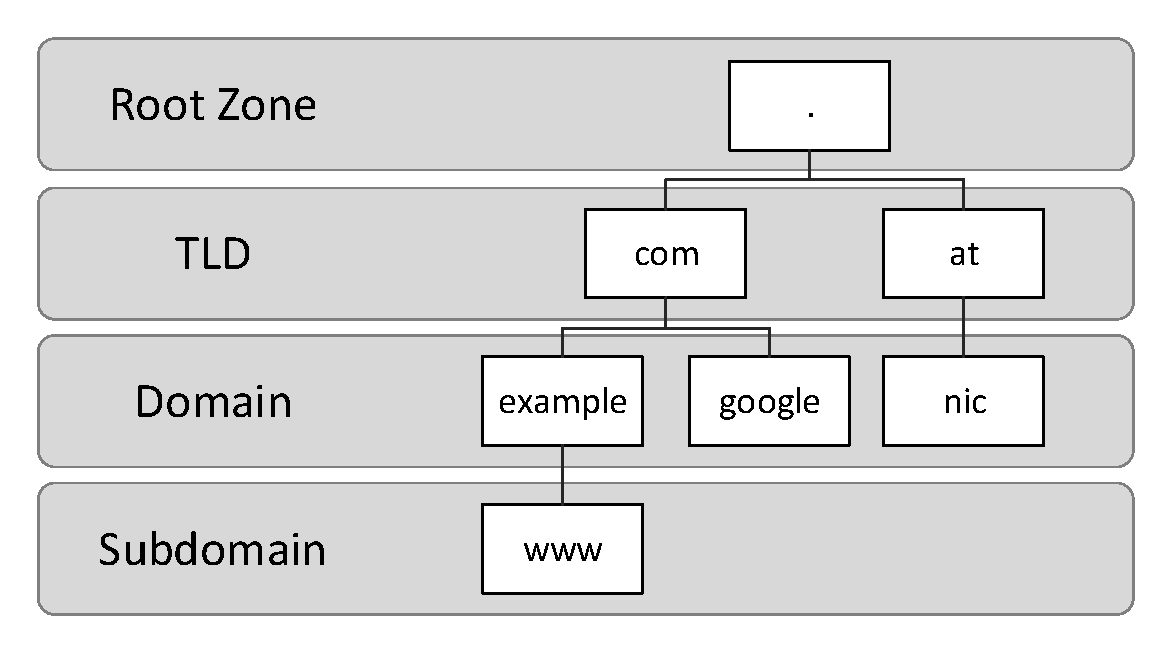
\includegraphics[width=0.5\textwidth]{DNS_NameSpaceLayers}
    \caption{Aufbau des DNS}
    \label{img:dnsnamespace}
\end{figure}

\section{Ressource Records, Sets und Zonen}

Alle Datensätze in DNS werden in einer als \textit{Ressource Record} (RR) bezeichneter Datenstruktur abgelegt. Ein RR besteht dabei aus 5 Informationen: Namen, Time-To-Live (TTL), Klasse (Class), Typ (Type), Datenfeld (Data). Dabei sind die Felder TTL und Class optional. Die Menge an Einträgen mit gleichen Werten der Felder Name, TTL, Class und Type bilden dabei ein \textit{Ressource Record Set} (RRset) \cite{rfc2181}, das kleinstmögliche abfragbare Element in DNS. Alle RR die einem definierten, zusammenhängenden Teil des DNS Namensraum zugeordnet sind, werden als Zone bezeichnet. Diese Sammlung an RR wird in einer Datei, dem \textit{Zone File}, gespeichert und von DNS-Server-Implementationen als Datenbasis genutzt.   

Wie in Listing \ref{lst:dnsZoneFile} zu sehen ist, werden die Daten in einem menschenlesbaren Format gespeichert. Zeile 1 enthält die Anweisung den Namens \texttt{test.example.com.} zu den IPv4-Adressen \texttt{172.30.0.7} und \texttt{172.30.0.8} aufzulösen. Zeile 3 fügt dem Namen weiter Information im Freitextformat hinzu. Zeile 1 und 2 bilden zusammen ein RRset für \texttt{test.example.com 3600 IN A}.

\lstinputlisting[caption={Ausschnitt aus dem Zone-File \textit{example.com}}, label={lst:dnsZoneFile}]{code/example-zone.txt}

\section{DNS Server}
\label{sec:dnsserver}

Um die globale, verteilte Datenbank des DNS nutzen zu können, ist es notwendig, dass diese den DNS-Client-Programmen zugänglich gemacht wird. Das Netzwerkprotokoll ist nach dem klassischen Client-/Server-Konzept ausgestaltet. Es erfordert keinen Verbindungsaufbau und verwendet einen einfachen, sequenziellen Ablauf an Anfragen und Antworten. Ein Client stellt dabei immer nur Anfragen an Server und verarbeitet deren Antwort. DNS-Server können hingegen, je nach Typ, auch selbst Anfragen an andere Server stellen und sind somit nicht nur auf das Beantworten von Anfragen beschränkt. Es können dabei vier unterschiedliche DNS-Server-Typen festgemacht werden.

\paragraph{Stub Resolver}
Die Software, die auf jedem Client-Rechner DNS-Anfragen von Programmen entgegennimmt und diese an die DNS Infrastruktur zur Auflösung übergibt, werden als \textit{Stub Resolver} bezeichnet. Diese können nach außen ausschließlich mit rekursiven Resolvern kommunizieren und nehmen selbst keine DNS-Namensauflösung vor. In manchen Fällen verfügen sie jedoch über einen Cache oder können aufgrund lokaler Policies (z.B. einem Hosts-File) eine Namensauflösung auf anderem Wege durchführen.

\paragraph{Rekursive Resolver}
\textit{Rekursive Resolver} (Recursive Resolver) sind spezielle DNS-Server die von Clients genutzt werden um Namen aufzulösen. Sie verfügen meistens über keine eigenen Zonen und sind damit als Vermittlungskomponente zwischen Endgeräten und den im Internet verfügbaren DNS-Servern zu verstehen.

\paragraph{Autoritative Server}
Server deren Hauptaufgaben im Auflösen von Namen einer oder mehrerer bestimmter Zonen besteht, werden \textit{autoritative Server} (auch Authoritative Server) genannt. Die Bezeichnung spiel auf den Umstand an, dass die Antworten dieses Servers die finale Wahrheit über die von ihm verwalteten Zonen darstellt. Sie lesen die Antworten direkt auf dem Zonen-File der entsprechenden Zone und verlassen sich nicht auf Antworten anderer Server oder Caches. Autoritative DNS-Server stellen damit die Endpunkte der Auflösung für die jeweiligen Domänen dar.

\paragraph{Forwarding DNS Server}
Eine spezielle Form des Rekursive Resolver wird als \textit{Forwarding DNS Server} oder \textit{Forwarding Resolver} bezeichnet. Aus Sicht des Stub Resolvers verhält er sich wie ein gewöhnlicher Rekursiver Resolver. Der Unterschied besteht darin, dass er selbst keinen Auflöse-Prozess durchführt- Die Anfragen werden lediglich an einen anderen Server weiterleitet, welche die eigentliche Auflösung durchführen. Die Ergebnisse werden meist gecacht bevor sie an den Client weitergegeben werden. Dies ist der Grund warum diese Server in seltenen Fällen auch als \textit{DNS-Netzwerk-Cache} oder \textit{Cache-Only Resolver} bezeichnet werden. 

\section{DNS Namensauflösungsprozess}
\label{sec:dnsresolution}

Der Namensauflösungsprozess erfolgt über mehrere Schritte und kann am besten anhand eines Beispiels dargestellt werden. Nehmen wir an, eine Applikation möchte die IPv4-Adresse des Namen \texttt{example.com} herausfinden und stellt eine Anfrage an den lokalen Stub Resolver (kurz stub) des Client. Der Prozess in Abb. \ref{img:dnsresolution} visualisiert und kann Schrittweise wie folgt beschrieben werden:

\begin{enumerate}
    \item Der stub stellt eine Anfrage nach dem Type A Record der Domäne example.com an den für ihn konfigurierten rekursiven Resolver.
    \item Der Resolver empfängt die Anfrage und prüft seinen lokalen Cache nach dem Eintrag. Da er diesen nicht aufgefunden wird fortgefahren.
    \item Nun startet der Resolver den rekursiven Auflösungsvorgang. Geht man von einem leeren Cache aus, wird mit der Root-Zone (.) begonnen. Die Anfrage nach www.example.com wird dafür an einen der 13 vorkonfigurierten Root-DNS-Server gesendet.
    \item Der Root-Server empfängt die Anfrage, kann jedoch nur den TLD Teil der Antwort auflösen. Es sendet daher die Adressen des autoritativen Nameserver für die TLD .com zurück.
    \item Der Resolver verarbeitet nun die Adressen und sendet die Anfrage an einen der autoritativen Server der .com Domäne.
    \item Der TLD Nameserver empfängt die Anfrage und prüft, ob für die Domäne example.com eine entsprechende Delegation existiert. Da diese in Form mehrerer NS Einträge vorliegt, wird eine Liste an autoritativen Nameserver-Adressen der SLD Domäne example.com als Antwort gesendet.
    \item Da nun die Adresse eines autoritative Servers für die vollständige Zieldomäne example.com gefunden wurde, kann die gewünschte Information abgefragt werden. Der Resolver sendet also ein letztes mal die Anfrage des Client, jetzt an den Nameserver der SLD example.com.
    \item Der autoritative Server der SDL example.com nimmt die Anfrage nach dem RR mit Typ A für die Domäne example.com entgegen und liefert nun die gewünschte Information in Form einer IPv4 Adresse.
    \item Der rekursive Resolver empfängt die Antwort, überträgt sie in seinen Cache und sendet dem anfragenden stub die IPv4 Adresse zurück.
\end{enumerate}

\begin{figure}[htbp]
    \centering
    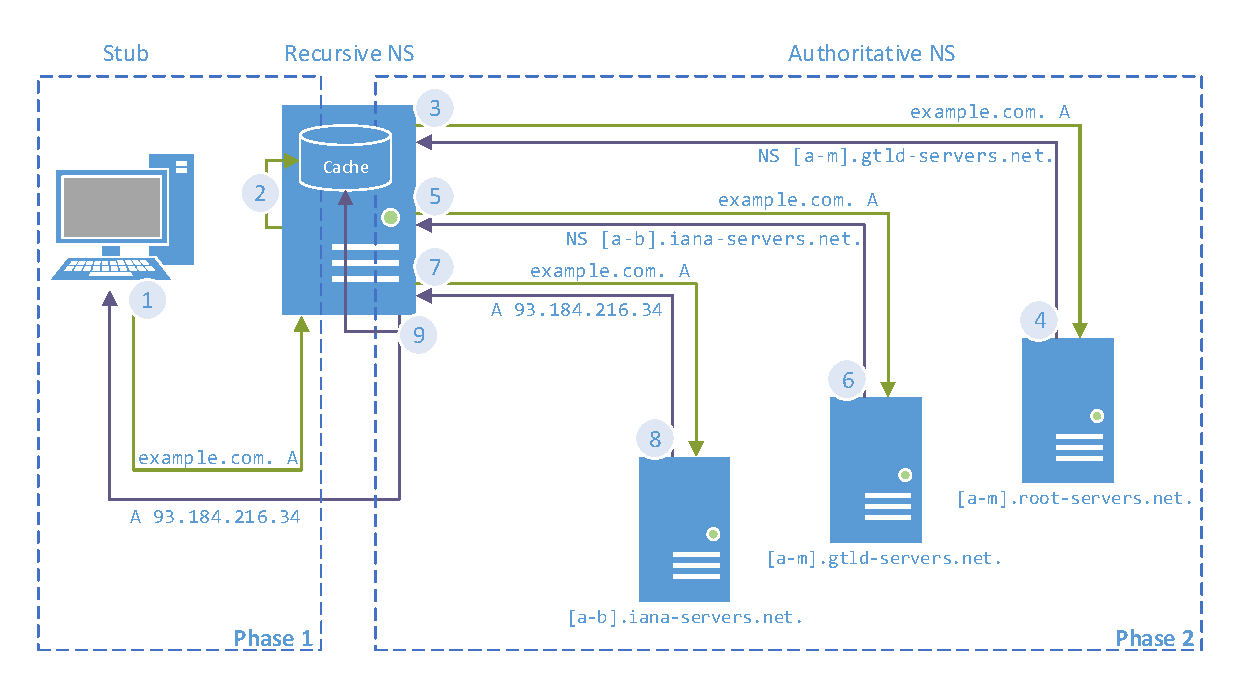
\includegraphics[width=\textwidth]{DNS_Resolution}
    \caption{Der schrittweise dargestellte Auflösungsprozess des Namen \texttt{example.com} über DNS. Der zeitliche Ablauf wird über die nummerierten Markierungen angezeigt.}
    \label{img:dnsresolution}
\end{figure}

\section{DNS Security}
\label{sec:dnssecurity}

Obwohl oder gerade weil DNS eines der grundlegendsten Services im Internet darstellt wurde bei der Spezifikation des Netzwerkprotokolls bewusst auf eine Authentifizierung verzichtet. Dies ist auf die Idee einer öffentlich zugänglichen, globalen Datenbank, nach dem Vorbild eines globalen Telefonregisters, zurückzuführen. Die Datenbasis der Namensauflösung wurde somit als frei öffentlich zugänglich definiert. Abgesehen davon, stammt das Protokoll aus einer Zeit in der modernen Schutzzielen wie Sicherheit und Vertraulichkeit wenig Beachtung geschenkt wurde. Dies führten zu einer Vernachlässigung des Sicherheitsgedanken und hat sich über die Zeit zu einem ernstzunehmenden Problem entwickelt. Verschärfend kommt hinzu, dass kein allgemeiner Konsens über die Sicherheitsziele herrscht. Dies Erschwert die Entwicklung einer Lösung und hat zu den unterschiedlichsten Ansätzen und Technologien geführt \cite{Grothoff2018}. Die übergeordneten Lösungskonzepte werden in Kapitel \ref{chap:solutions} näher behandelt.

\section{Resolver Position}
\label{sec:dnsresolverposition}
Der Aufbau der Client-nahen Infrastruktur spielt eine wichtige Rolle für die Sicherheit des Clients. Wie im Abschnitt \ref{sec:dnsresolution} beschrieben, wird vom Client einen Recursive Resolver benötigt um die eigentliche Auflösung der Namen durchzuführen. Die Lage dieser Komponente im Netzwerk ist dabei vor allem für Privacy ausschlaggebend. Es existieren insgesamt 5 mögliche Positionen die ein Recursive Resolver einnehmen kann\cite{VanHeugten2018} (siehe Abbildung \ref{img:dnsresolverposition}):

\paragraph{Local Recursive Resolver}
Ist der Recursive Resolver im Netzwerk des Clients positioniert und wird die selbe öffentliche IP-Adresse zur externen Kommunikation benützt, spricht man von einem \textit{Local Recursive Resolver}. Da dieser in den meisten Fällen unter der Kontrolle des Benutzers steht und auch nicht von Dritten überwacht wird, ist es unbedenklich, dass Anfrage und Client-IP einfach ausgelesen werden können. Da für den rekursiven Auflöse-Prozess jedoch die selbe Adresse wie der Client verwendet wird, ist es für Betreiber von autoritative DNS-Server einfach eine Verbindung zwischen Anfrage und User herzustellen.  

\paragraph{Private Recursive Resolver}
Unter \textit{Private Recursive Resolver} können alle Resolver zusammengefasst werden, die zwar unter der Kontrolle der nutzenden Personen steht, aber nicht die selbe Adresse für die Kommunikation verwendet. Da die autoritativen DNS-Server nur von der Resolver-Adresse aus angesprochen werden, ist keine Verknüpfung zur Client-Adresse mehr möglich. Die hilft der Privacy jedoch nur, wenn die Adresse des Servers nicht trotzdem einer einzelnen Person zugeordnet werden kann.

\paragraph{ISP Recursive Resolver}
Die Mehrheit der Nutzenden im privaten oder einzelunternehmerischen Umfeld verwenden den Resolver ihres Internet Service Providers (ISP). Diese \textit{ISP Recursive Resolver} werden von den Internetanbietern zur Verfügung gestellt um eine grundlegende Internetkonnektivität anbieten zu können. Diese Server sind in den meisten Fällen im Netzwerk des ISP positioniert und haben daher oft bessere Latenzzeiten als andere, über das Internet erreichbare, Resolver. Diese Resolver werden oft für das überwachen von Kundenaktivitäten und einspeisen von Werbeseiten verwendet \cite{Weaver2011}, was grundsätzlich gegen den Gedanken der Privacy verstößt.

\paragraph{Public Recursive Resolver}
Sogenannte \textit{Public Recursive Resolver} sind über ihre freie Zugänglichkeit definiert und haben je nach Fokus des Anbieters verschiedenste Regelungen was Privacy betrifft \cite{Prince2018}\cite{Quad92018}. Wird nun ein Anbieter mit speziellem Fokus auf Sicherheit und Vertraulichkeit gewählt, kann ein akzeptabler Grad an Privacy erreicht werden. Voraussetzung ist dafür die Sicherung der Übertragung zwischen Stub-Resolver und Recursive Resolver. Einige Projekte bieten dafür Unterstützung für spezielle Netzwerkprotokolle, die diesen Zweck erfüllen sollen (siehe dazu Kapitel \ref{chap:technologies}. Resolver die speziellen, selbst auferlegten Vorschriften zur Verbesserung der Informationssicherheit folgen werden auch als \textit{Trusted Resolver} bezeichnet, wobei diese öffentlich (Public) oder nur mit Authentifizierung (private) zugänglich sein können.

\paragraph{Local-Loopback Resolver}
Eine Sonderform stellt der \textbf{Local-Loopback Resolver} dar. Dieser wird direkt auf dem Client-Rechner installiert und ist nur für Programme auf eben diesem Host erreichbar. Dies führt zu dem Umstand, dass der Stub-Resolver keine, für das umliegende Netzwerk sichtbare Kommunikation mehr durchführt. Der Installierte Resolver löst die Anfragen dann entweder rekursiv über das Netzwerk auf oder fungiert als Forwarding Resolver (siehe Abschnitt \ref{sec:dnsserver}) und verhält sich somit wie ein Stub-Resolvers.

\begin{figure}[htbp]
    \centering
    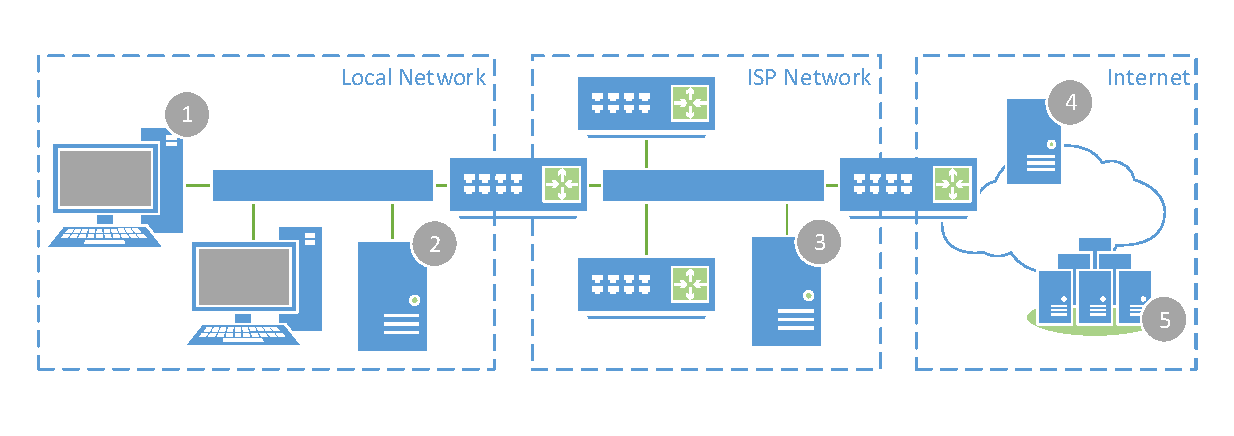
\includegraphics[width=\textwidth,trim={0 1cm 0 0.5cm},clip]{DNS_ResolverPosition}
    \caption{Zeigt die möglichen Positionen eines DNS-Resolvers. (1) Local-Loopback Resolver, (2) Local Recursive Resolver, (3) ISP Recursive Resolver, (4) Private Recursive Resolver, (5) Public Resolver}
    \label{img:dnsresolverposition}
\end{figure}


\chapter{Schwachstellen und Bedrohungen}
\label{cap:threads}

\todo[inline]{Bedrohungen sind schon zu detailliert ... Trennung in Schwachstellen, Bedrohungen, Angriffe? Einfach Kürzen?}

\section{Authentizität}
\label{sec:Thread-Auth}

Wie in den Anfängen des World-Wide-Webs und dessen Transportprotokoll HTTP ist auch bei der Konzeptionierung der DNS Protokolls keine Rücksicht auf Sicherheitsaspekte wie Integrität und Vertraulichkeit genommen worden. Da DNS nach RFC1035 auf jede Form von Authentifizierung verzichtet, ist auch ein Prüfen der Identität der jeweiligen Gegenstelle, sowie der eigentlichen Nutzdaten, nicht vorgesehen. Dies birgt jedoch eine hohe Anfälligkeit auf Man-in-the-Middle Attacken mit sich. Ein Angreifer, dem es gelingt, sich aus Sicht des Netzwerks, zwischen eine der beteiligten Komponenten zu positionieren, hat komplette Kontrolle über den Informationsfluss zwischen den betroffenen Geräten. Sollte sich der Angreifer zwischen Endgerät und Recursive Resolver befinden, kann jede DNS-Interaktion nach belieben manipuliert werden. Solle es dem Angreifer gelingen sich vor einem Authoritativem DNS-Server zu stellen, können alle Anfragen und Antworten an die von diesem Server bereitgestellten Domänen manipuliert werden. 

Die verteilte Natur von DNS sorgt zusätzlich dafür, dass Einträge für lange Zeit verändert werden können, ohne dass es eine einfache Form der Sanierung gibt. Dies ist dem Umstand geschuldet, dass der Angreifer den Wert der Time-To-Live (TTL), welcher die Lebenszeit der Eintrage im Cache anderer Server festlegt, beliebig verändern kann. Somit können Caching Resolver die eine sehr hohe maximale TTL konfiguriert haben über einen großen Zeitraum hinweg beeinflusst werden.

Wie in Abschnitt \ref{sec:DNS} beschrieben baut sich das DNS aus verschiedenen Zonen auf, die wiederum aus Einträgen (Resource Records; RR) bestehen. Obwohl das Format und der Aufbau der beschreibenden Zonen-Files klar spezifiziert ist, wurde im System keine Möglichkeit zur Prüfung der Authentizität vorgesehen. Somit ist es weder für die Server-Software noch für die empfangenen Clients möglich die Unversehrtheit und Quellenauthentizität der Einträge zu prüfen. Dieser Umstand stellt eine der zentralen Schwachstellen der aktuellen DNS Infrastruktur dar und ist Grundlage für verschiedenste Angriffe.

Eine weiter Angriffsmöglichkeit bietet das sogenannte \textit{BitSquatting}. Bei diesem Angriff werden zufällige Fehler im Speicher von Geräten ohne fehlererkennenden Speichermodulen ausgenützt \cite{Dinaburg2011}. Da es dadurch zu falschen Anfragen kommt, gibt es auch keine Möglichkeit sich auf Protokoll- bzw. System-Ebene zu schützen. Die einzige effektive Lösung stellt der Einsatz von \textit{Error-correcting code memory} Hardware dar.  

\section{Vertraulichkeit}
\label{sec:Thread-Priv}

Das Internet als globale, vernetzende Technologie, rück immer weiter in den Mittelpunkt der Telekommunikation. Damit verbunden ist der steigende Bedarf an Sicherheit und Schutz dieses Gesamtsystem. Die IETF behandelt dieses Thema in verschiedensten RFCs, wobei Privicy einen der Schwerpunkte darstellt. Mit der 2013 veröffentlichten RFC6973 \textit{Privacy Considerations for Internet Protocols} wurde der Grundstein für die aktive Förderung von vertraulicher Kommunikation im Internet gelegt \cite{Cooper2013}. 
Für den DNS Kontext wichtiger ist die darauf aufbauenden RFC7626 \textit{DNS Privacy Considerations}\cite{Bortzmeyer2015} welche die Relevanz von DNS Privicy klar macht. Im speziellen wird auf die notwendige Unterscheidung zwischen der freien Zugänglichkeit der DNS Daten an sich und der Öffentlichkeit der Anfragen aufmerksam gemacht. Das plakatives Beispiel wird die Website der Anonymen Alkoholiker genannt, die öffentlich Zugänglich ist, wobei die personenbezogenen Zugriffsdaten auf keinen Fall öffentlich gemacht werden dürfen. Da DNS in im ursprünglichen Konzept jedoch keine Unterscheidung macht, sind die Anfragedaten für alle Zwischenstellen einfach lesbar. Darüber hinaus, existiert kein Schutz der Vertraulichkeit der Übertragung, was es jeder Zwischenstelle das einsehen aller Anfragen und Antworten erlaubt.
Das Problem der fehlenden Transportsicherheit betrifft die Sicherheit des DNS allgemein, ein weniger behandeltes, jedoch für die Privicy ebenso relevantes Problem stellt die Vertraulichkeit der Anfragen selbst da. Trotz bestehendem Schutz des Transports wäre es vielen Stellen der DNS-Auflösungskette möglich die Anfragedaten mit Personen oder zumindest Clients zu verknüpfen. Dieser Umstand wird durch die in RFC7871 spezifizierte Technik \textit{EDNS0 Client Subnet} zusätzlich verschärft, da damit die aktiver Erhaltung kritischer Informationen durch die Komponenten möglich wird \cite{Contavalli2016}. Wie in der \textit{Privacy Note} der RFC7871 beschrieben sind solche Vorhaben jedoch mit größter Vorsicht und auf keinen Fall gegen den Willen der Nutzenden einzusetzen. Der 2017 eingebrachte Entwurf zum einführen einer ClientID\cite{Licht2017} wurde zur Unterstützung des Privicy-Gedanken nicht weiter verfolgt.

\section{Nutzung als DoS-Amplifier}
\label{sec:Thread-DosAmp}

Die Nutzbarkeit von DNS als Verstärker (Amplifier) von DoS Attacken ist schon länger bekannt und wurde auch schon früher als Problem erkannt \cite{ICANN2006}. Nach dem Anual Wordwide Infrastructure Security Report 2017 befindet sich DNS als Trägertechnologie von DoS-Attacken auf Platz 1 \cite{Alcoy2017}. Die leichte Ausnutzbarkeit und schlechte Zurückverfolgbarkeit macht DNS neben NTP zu den beliebtesten Verstärkungsmethoden. Wie Anagnostopoulos et al.\cite{Anagnostopoulos2013} und van Rijswijk-Deij et at.\cite{VanRijswijk-Deij2014} zeigen konnte besteht darüber hinaus das Problem, dass DNSSEC die Situation bei steigender Verbreitung weiter verschärft. Mithilfe von DNSSEC konnte ein durchschnittlichen Verstärkungsfaktor von 47,2 erreicht werden, wobei die maximale Verstärkungsrate bei DNS ohne DNSSEC bei 12,8 liegt. Dieser Umstand ist auf die mit DNSSEC eingeführte Erweiterung EDNS0 zurückzuführen, die es ermöglicht Antworten, die größer als die ursprüngliche Grenze von 512 bytes sind, zu empfangen. Es konnte gezeigt werden, dass 90\% der offenen Resolver maximale Packetgrößen von 4k bytes unterstützen, was bei einer Anfragegröße von 40 byte einen maximalen Verstärkungsfaktor von 102,4 zulassen würde. Dies birgt zusammen mit anderen Kritikpunkten ein massives Hemmnis für die Verbreitung von DNSSEC und ist unter anderem ein Grund für die schlechte Verbreitungsrate. Das Kernproblem liegt hier jedoch an dem eingesetztem Transportprotokoll UDP zusammen mit dem Umstand, dass DNS keinerlei Authentifizierung des Clients verlangt. Betrachtet man andere Protokolle mit ähnlichen Bedingungen (z.B. NTP) zeichnet sich ein ähnliches Bild. Der Vorwurf an DNSSEC als Verursacher der DoS-Amplifikation Problematik ist somit kritisch zu betrachten.


\chapter{Angriffe}
\label{chap:attacks}

Die meisten DNS-Sicherheitsrichtlinien richten sind an Betreiber von extern gerichteten Installationen. Das Thema \textit{DNS Client Security} wird wenn nur am Rande behandelt. Der nachfolgende Abschnitt befasst sich daher von allem mit Bedrohungen der Interaktion zwischen DNS-Resolver und rekursivem DNS-Server. 
Es gibt dabei zwei grundlegende Möglichkeiten einen DNS-Client anzugreifen: Über direktes kommunizieren mit der Netzwerkschnittstelle des Clients oder mittels Angriff auf einen Teil der Client-nahen Infrastruktur. Um die Auswirkung klar ersichtlich zu machen wird in Abschnitt \ref{sec:Attacks-Summary} eine tabellarische Zusammenfassung mit den verletzen Sicherheitskriterien (nach CIA-Triade) gegeben. 

% Trennung wirklich sinnvoll?

\section{Direkte Angriffe}

Angriffe die das Verhalten einzelner DNS-Clients über eingreifen in deren Kommunikationsfluss beeinflussen, können als \textit{direkte Angriffe} zusammenfasst werden. Diese Verfahren sind nur effizient wenn der Angreifer entweder passiv (Sniffing) oder aktiv (Man-in-the-middle) an der Netzwerkverbindung des Clients beteiligt ist. 

\subsection{DNS Sniffing und Spoofing}
% Sniffing / Spoofing zusammenlegen?

Als Sniffing Angriffe werden, nach CAPEC, alle Arten von Angriffen bezeichnet die es ermöglichen Nachrichten zwischen mindestens 2 Parteien zu beobachten, mitlesen und/oder mithören. (https://capec.mitre.org/data/definitions/157.html). Im Kontext DNS hat dies eine spezielle Bedeutung da es, aufgrund des fehlenden Schutz der Vertraulichkeit, ermöglicht, alle Informationen der Anfragen und Antworten einzusehen. Somit ist das Kommunikationsverhalten der Opfergeräte leicht nachzuvollziehen, was zum Beispiel den Recon-Schritt der Cyber-Kill-Chain (siehe \ref{sec:dnssecurity}) erheblich erleichtert. 

In IP-Netzen gibt es verschieden Möglichkeiten eine Sniffing Attacke durchzuführen: 

Eine Möglichkeit ist der Angriff der Netzwerkhardware. Bei einem Hub als Netzwerkverteiler erhalten immer alle angeschlossenen Teilnehmer alle Pakete. Es können daher die Pakete aller anderen an diesem Hub angeschlossenen Geräte einfach mitgelesen werden. Wird ein Switch einsetzt wird für jeden Anschluss (Port) die MAC-Adresse des angeschlossenen Geräts in eine Tabelle eingetragen. Es werden somit nur noch Pakete mit passender MAC-Adresse an die entsprechenden Ports weitergeleitet. Ein Angreifer kann bestimme Switches jedoch durch künstliche Füllen der MAC-Switching-Tabelle (MAC-Flooding Angriff) in ein, einem Hub ähnliches, Verhalten zwingen. Soll ein spezielles Endgerät mit bekannter MAC-Adresse angegriffen werden, kann bei anfälligen Switches auch ein MAC-Duplication Angriff durchgeführt werden. Dabei sendet der Angreifer Pakete mit der gefälschter MAC-Adresse des Opfers was den Switch dazu verleitet die Adresse auf zwei Ports einzutragen. Anfällige Switches senden daraufhin die Pakete des Opfers auch auf den Port des Angreifers.

Ist die Netzwerkhardware nicht angreifbar bleibt noch die Möglichkeit den Netzwerkstack der Client-Geräte zu attackieren. Hier kann eine Schwäche im \textit{Address Resolution Protocol} (ARP) ausgenützt werden. Dieses Protokoll ist für die Auflösung von logischen Adressen (z.B. IP-Adressen) zu Adressen der Hardware (MAC-Adresse) verantwortlich (https://tools.ietf.org/html/rfc826). Da ARP stateless konzeptioniert wurde und auch keine Art von Authentifizierung verlangt kann eine als \textit{ARP Spoofing} bekannte Attacke durchgeführt werden. Mit dieser kann die Zuordnung zwischen MAC-Adresse und logischer Adresse (z.B. IP-Adresse) im lokalen Netzwerk bewusst manipuliert werden. Damit ist es einem Angreifer leicht möglich sich als vertrauenswürdiger Host des Netzwerks auszugeben. Wird die MAC-Adresse des Netzwerk-Gateways mit der eines abhörenden Rechners getauscht ist auch ein umfangreiches Abhören des Netzwerkverkehrs möglich.

% Da es Ethernet-Broadcasts zur Kommunikation einsetzt, somit Verbindungslos ist und keinerlei Form von Authentifizierung verlangt, kann ein Angreifer jede MAC-Adresse als Antwort auf die Frage nach jeder beliebigen IP-Adresse senden. Dies setzt natürlich die selbe Layer-2 Broadcast-Domain und das fehlen entsprechender Schutzmaßnahmen voraus. Gelingt das Eintragen einer gefälschten MAC-Adresse, werden alle Pakete die an die IP-Adresse des Ziels gesendet werden an die Maschine mit der gewählte MAC-Adresse geschickt. Wird nun die Hardware-Adresse des default Gateway gegen die des Angreifers getauscht, ist es diesem Problemlos möglich den gesamten Netzwerkverkehr außerhalb des lokalen Subnetzes mitzuschneiden und zu verändern.  

Eine weitere Möglichkeit sich als gefälschter Gateway zu positionieren ist es das \textit{Dymamic Host Configuration Protocol} (DHCP) mittels \textit{DPHC-Spoofing} auszunutzen. Bei diesem Angriff wird ein eigener DHCP-Server im Subnet des Opfers positioniert. Dieser gibt zwar gültige IP-Adressen aus, verändert aber die default Gateway und/oder die DNS Server Einstellungen. Somit kann ein Host des Angreifers als Gateway oder DNS-Resolver zwischengeschalten werden und den Netzwerkverkehr kontrollieren. Da DHCP wie ARP auf Ethernet-Broadcasts ohne Authentifizierung setzt sind die Schwachstellen sehr ähnlich. Da der attackierte Client jedoch auch das Annahmen der gefälschten Sitzung über Broadcast verteilt ist das Erkennen etwas einfachen als vom ARP-Spoofing. 

Eine spezielle Methode zum umlenken der Netzwerkpakete stellt das ein Angriff auf das \textit{Internet Control Message Protocol} (ICMP) dar. Dieses Protokoll dient als Grundlage für verschiedenste Unterstützungsaufgaben in IP-Netzen. Am bekanntesten ist die ICMP-Ping Funktion, mit der sich die Konnektivität von Hosts prüfen lässt. Obwohl ICMP oft auf diese Funktionalität reduziert wird beinhaltet es eine Vielzahl von teils wenig bekannten Aufgaben. Die, in Hinblick auf Sniffing, relevante Schwachstelle verbirgt sich dabei in der ICMP-Redirect Funktion, welche für Optimierung des Routing-Prozesses vorgesehen ist. 

Außerdem wird DNS hauptsächlich über UDP verwendet, was ein fälschen (spoofing) der Absenderadresse trivial macht. Da dadurch auch die Transaktions ID und das Absendeport bekannt wird, kann der Angreifer sofort ein gefälschtes Antwortpacket senden und somit den Eintrag der abgefragten Domäne im Resolver des Ziels beliebig verändern oder erweitern. Durch das setzen von hohen TTL Werten kann dieser Zustand lange über die physische Präsenz des Angreifers hinaus aufrecht erhalten werden.

\todo[inline]{Sniffing und Spoofing klar auftrennen?!}

\subsection{DNS Rebinding}

\todo[inline]{DNS Rebinding kurz beschrieben (weil schon Angesprochen)}

\section{Indirekte Angriffe}

\subsection{Reliance Upon Transitive Trust}

\todo[inline]{Angriff über Trust Reliance beschreiben}

\begin{draft}
\begin{markdown}
* Unbemerkte übernehme von Domänen möglich
* Kompromittierung von Stakeholder-Diensten möglich
  * Bei Websites  (HTTP od. uralt Browser mit Mixed Active Content) führt die Kompromittierung eines einzigen Ressourcenservers zum Kompromittierung der gesamten Seite: XSS wird einfach möglich wenn z.B. eine JS-Datei eines Werbeanbieters in die Seite geladen werden kann.
  * Wenn eine einzige aktive Ressource über http nachgeladen wird oder für TLS Attacken (Poodle, ) anfällig ist, kann die Seite und somit der Client angegriffen werden.
* Bei nicht verschlüsselten Netzwerkprotokollen (plain SMTP/POP3/IMAP, FTP, MQTT) kann die Verbindung vollständig übernommen werden.
* In jedem Fall sorgt eine erfolgreiche Attacke zum Übergang der Verfügbarkeitskontrolle an den Angreifer (bis zum Erkennen das Problems und entfernen der eingeschläuschten Einträge)
\end{markdown}
\end{draft}

\subsection{Name Collisions and Leaked Queries} 

\todo[inline]{Leaked Queries wirklich relevant? Vielleicht für Quellen Authentizität?}

\begin{draft}
  \begin{markdown}
* Durch eigene interne TLDs (z.B. .local) kann es zu Kollisionen im globalen Namespace kommen (new TLDs).
* Mögliche Kollisionen können bewusst ausgenutzt werden.
* Durch falsch/schlecht konfigurierte DNS-Resolver können interne Anfragen zu externen DNS-Servern getragen rden -> Information Disclousure
* Speziell bei "home-use" und ohne "LockDown" kann durch lokale Proxies und Resolver von "leakage" betroffen sein. Auch BYOD-Geräte speziell gefährdet wenn durch falsche Konfiguration DNS-Anfragen zum Auflösen internen Ressourcen an externe DNS-Server gestellt werden.
\end{markdown}
\end{draft}

\subsection{C\&C/Exfiltration über DNS Tunneling}

\todo[inline]{Überlegen ob DNS Tunneling wirklich reinpasst}

\begin{draft}
  \begin{markdown}
* Mit allen "offenen" resolvern nutzbar
* Bei "best-practice"-Einstellungen des resolvers sehr langsam
* Nicht einfach zu erkennen
* Für sehr kleine Datenmengen durchaus zuverlässig (C\&C)
* KillChain: Data Exfiltration, Controll
\end{markdown}
\end{draft}

\subsection{DoS-Amplification Angriff}
\label{sec:attack-dosamp}

\todo[inline]{DoS Angriff schreiben}

\begin{draft}
Durch DoS von Resolvern oder DNS-Servern können kritischen Unternehmensdienste kurzfristig außer Betrieb genommen werden. Da die Verbindung zwischen diesen hoch vernetzten Diensten stark von DNS abhängt hat der Ausfall eines einzigen zentralen Dienstes (DynDns Vorfall) schwerwiegende Auswirkungen auf alle anhängenden Dienste.
\end{draft}

\todo[inline]{DoS Angriff schreiben}

\subsection{BitSquatting}

Eine weiter Angriffsmöglichkeit bietet das sogenannte \textit{BitSquatting}. Bei diesem Angriff werden zufällige Fehler im Speicher von Geräten ohne fehlererkennenden Speichermodulen ausgenützt. Es konnte gezeigt werden, dass es durch solche Fehler zum stellen fehlerhafter Anfragen an potenziell existente Domänen kommen kann\cite{Dinaburg2011}. Dieser Effekt kann nun bewusst ausgenutzt werden indem eine große Anzahl an Domänen registriert werden, deren Name sich nur um ein Bit von viel besichten Domänen unterscheidet (siehe Listing \ref{lst:bitquatting}). Da es dadurch zu falschen Anfragen kommt, gibt es auch keine Möglichkeit sich auf Protokoll- bzw. System-Ebene zu schützen. Die einzige effektive Lösung stellt der Einsatz von \textit{Error-correcting code memory} Hardware dar.  

\begin{lstlisting}[caption={Drei mögliche BitSquatting-Domänen für die Zieldomäne \texttt{amazon.com}}, label={lst:bitquatting}]
amazon.com = 61   6d   61 7a   6f   6e 2e 63 6f 6d
           ... 01101101 ... 01101111 ... 
aeazon.com = 61   65   61 7a   6f   6e 2e 63 6f 6d  
           ... 01100101 ...
                   ^
a-azon.com = 61   e2   61 7a   6f   6e 2e 63 6f 6d 
           ... 00101101 ...
                ^
amazgn.com = 61   6d   61 7a   67   6e 2e 63 6f 6d
                        ... 01100111 ...
                                ^
\end{lstlisting}

\section{Übersicht}
\label{sec:Attacks-Summary}

\todo[inline]{Angiffszusammenfassung schreiben. (Nicht sicher ob notwendig)}

\chapter{Lösungsansätze}
\label{chap:solutions}
% Noch nicht auf spezielle technische Lösungen eingehen!

\section{Authentizität der Records}
\label{sec:Solution-RecordAuth}

Wie in Kapitel \ref{sec:Thread-Auth} beschrieben wurde, ist die Authentizität der RR ein zentrales Problem in DNS. Zur Lösung wurde schon früh der Einsatz kryptografischer Signaturen postuliert. Mithilfe dieser könnten alle Einträge bei der Erstellung signiert, zusammen mit den Signaturen übertragen und dann von der Gegenstelle validiert werden. Dadurch wird es möglich die Integrität und Authentizität der empfangenen Einträge eindeutig sicherzustellen. Werden die Zonendateien nur bei Änderung signiert und der private Schlüsselteil anschließend wieder entfernt, besteht sogar die Möglichkeit Server-Konfigurationen vor ungewollter Veränderung zu schützen. 
Die zentralen Fragen sind dabei, wie bei allen Signaturverfahren, das Schlüsselmanagement und die damit verbundene Vertrauensstellung zwischen den einzelnen Parteien. Das notwendige Vertrauen kann dabei auf verschiedenste Wege erreicht werden. Die gängigsten Methoden sind \textit{Chain-of-trust}, \textit{Web-of-trust}, \textit{Shared Key} und \textit{Trust-On-First-Use} (TOFU). Wie im folgenden Kapitel beschrieben wird, beantworten die unterschiedlichen Technologien diese Frage auf diverse weise, wobei zumindest TOFU als unzureichend Sicher eingestuft werden kann \cite{Wendlandt2008}.
Des weitern ist zu erwähnen , dass die Integrität der Nachrichten trotz Signatur nicht immer garantiert werden kann. Einige Signaturmechanismen, konkret die darin genützten Hash-Algorithmen, weisen bekannte Schwächen aus, die bei einem Angriff ausgenützt werden können. Modernes Beispiel stellt dabei der Angriff \textit{Shattered} auf den SHA-1 Algorithmus dar \cite{Stevens2017}. 

\section{Authentizität der Endstelle}

In Kapitel \ref{sec:Thread-Auth} wurde erwähnt, dass es in DNS-Netzwerkprotokoll keine Möglichkeit gibt die Authentizität der Gegenstelle zu prüfen. Abhilfe für dieses Problem schafft einerseits das zuvor besprochene kryptographische Signieren der Einträge, da so bei einem Eingriff keine unbemerkte Modifikation des Inhalts möglich ist. Dieser Schutz scheitert jedoch an der praktischen Umsetzung, da es einen Fallback-Mechanismus ausschließen müsste, da ansonsten eine Downgrade-Attacke möglich wäre. Bei diesem Angriff werden die die Signaturen aus dem Antwort-Paket entfernt, was bei einem Client zu dem Eindruck führt, dass der Server die Unterstützung von Signaturen eingestellt hat. Die meisten Implementierungen würden diesen Umstand ignorieren und somit die potenziell gefälschten Antworten akzeptieren.  

Der erste Schritt zur Lösung dieses Problem stellt das einführen eines Authentifizierungsverfahren dar. In den meisten Fällen wird dafür eine asymmertischer Kryptografie basierende Methode eingesetzt. Dieses besteht aus 2 Schritten: Als erstes teilt die fragliche Endstelle seinen öffentlichen Schlüssel mit, der Client trifft nun eine Entscheidung ob er dem Schlüssel vertraut oder nicht. Wir schon in Abschnitt \ref{sec:Solution-RecordAuth} erwähnt, gibt es dafür verschiedene Methoden um das notwendige Vertrauen zu dem gegebenen Schlüssel herzustellen und zu prüfen. Der zweite Schritt stellt sicher, dass die Endstelle auch im Besitz des passenden, privaten Schlüssels ist. Dabei wird oft die Authentifizierung und die Sitzungsschlüsselübertragung zusammengefasst. Der Client überträgt dabei seinen Informationsteil für die Sitzungsschüsselerstellung verschlüsselt mit dem öffentlichen Schlüssel des Gegenübers. Eine erfolgreiche Aushandlung des Sitzungsschlüssels ist damit nur möglich wenn die Endstelle die Nachricht auch entschlüsseln kann, was nur mit passendem privaten Schlüssel möglich sein sollte. 

\section{Vertraulichkeit der Verbindung}

Obwohl die Integrität und Authentizität der Nachrichten eines der größten Probleme für DNS darstellt, ist speziell DNS-Privicy zu einem wichtigen Thema geworden. Die nachhaltige Lösung zur Sicherstellung der Vertraulichkeit ist, wie damals auch bei HTTP, der Einsatz einer geeigneten Verschlüsselungstechnologie. Auf welcher Ebene diese Stattfindet ist dafür grundsätzlich nicht relevant. Der Einsatz von etablierten Technologien wie TLS liegt jedoch nahe, obwohl für DNS auch eigene Lösungen entwickelt wurden. So stellt der Umstand, dass DNS primär auf UDP aufbaut eine Hürde beim Einsatz von TLS dar, welches ein verbindungsorientiertes Protokoll wie TCP vorschreibt.

\section{Vertraulichkeit der Anfragen}
\label{sec:solutions-PrivRequest}

Ein in der Vergangenheit wenig beachtetes Problem ist die Vertraulichkeit der Anfragen selbst und damit das notwendige Vertrauen an die Betreibenden der DNS-Infrastruktur selbst. Speziell Rekursive Resolver von großen ISPs akkumulieren eine große Menge an DNS-Daten, welche auf vergleichsweise einfache Art zur Nachvollziehung von Kommunikationsverläufe der Nutzenden herangezogen werden kann. Zum umgehen dieser Schwachstelle gibt es zwei getrennte Entwürfe.

Auf der einen Seite gibt es Vorschläge die darauf abzielen personenbezogene Informationen wie die IP-Adresse bewusst von den Anfragedaten zu trennen. Dafür wird der Umstand ausgenützt, dass es möglich ist die Anfragen- und Antwortdaten von den Kommunikationsdaten zu trennen. Dies wird durch einen, für den Recursive Resolver transparente, Ende-zu-Ende-Verschlüsselung zwischen Stub Resolver und einem speziellen DNS-Server möglich. Der DNS-Server entschlüsselt dabei die erhaltene Anfrage und löst diese rekursiv auf, verschlüsselt die Antwort und sendet diese an der Recursive Resolver zurück, welcher die Antwort an den Client weiterreicht. Durch dieses Verfahren kann der Recursive Resolver weder Anfrage noch Antwort lesen, wobei der eigentlich auflösende Server zwar die Daten aber keinen Hinweis auf die Identität des Client erhält.

Ein komplett anderer Entwurf basiert auf der Ablöse des DNS als Gesamtheit, da davon ausgegangen wird, das DNS, aufgrund seines Grundkonzepts, nie strengen Ansprüchen auf Vertraulichkeit genügen wird. Diese Alternativkonzepte bauen die für ein Namensauflösungssystem notwendige verteile Datenbank mithilfe von Technologien wie Dirstibute-Hash-Tables (DHT) oder Public Ledger auf Blockchain-basis auf. Da diese Lösungsentwürfe radikal vom bestehenden Konzept des DNS abweichen, werden sie hier nicht weiter behandelt.      

\todo[inline]{Kurze Anmerkung über VPN / TOR / etc. => Langsam, usw. (Steht in irgendeinen Paper -> Referenz)}

\section{Einsatz eines verbindungorientierten Transportprotokolls}

Über die Zeit sind verschiedenste Lösungsvorschläge zum, in Abschnitt \ref{sec:Thread-DosAmp} behandelten, Problem der DoS-Verstärkung ausgearbeitet worden. Die einfachste Möglichkeit einer Lösung besteht im Ablösen des Verbindungslosen UDP zugunsten eines Verbindungsorientierten Protokolls wie TCP. Der notwendige Verbindungsaufbau könnte im Falle eines klassischen IP-Spoofings nicht abgeschlossen werden, was das Stellen einer Anfrage verhindern würde. Damit wäre DNS nicht mehr als Verstärker nutzbar. Die Nachteile dieser Lösung bestehen jedoch in ihrem Vorteil, da der Verbindungsaufbau viel Zeit in Anspruch nimmt und zusätzliche Ressourcen auf dem Server binden würde. Wie Zuh et al. \cite{Zhu2015} jedoch feststellen konnte, ist die Auswirkung auf die Performance in den meisten Fällen jedoch stark überschätzt. In seiner Arbeit wurde festgestellt, dass bei einer TLS Verbindung wischen Stub-Resolver und Recursive Resolver lediglich 21\% Zeitverlust auftritt, wobei die Ressourcenerhöhung bei den meisten Resolvern vernachlässigbar ist.

\section{Härten des Resolvers}

\begin{draft}
\begin{markdown}
* Source Port randomization
* ACLs am Resolver
* In-Domain check for Glue Records
* 0x20
* TXID Redomization
* TTL min. 
\end{markdown}

(https://tools.ietf.org/html/rfc545)

\end{draft}


\chapter{Technische Umsetzungen}
\ref{chap:technologies}
% Kurzbeschreibung, Löst welches Problem?, Vorteile/Nachteile, Verbreitung
% Mehr Struktur? Bilder?!

\section{DNSSEC}

Wie in \ref{sec:DNSSecurity} ausführlich beschrieben, erfüllt des DNS System selbst keinerlei Schutzziele der Informationssicherheit. DNSSEC, als eine Sammlung an IETF-Spezifikationen, erweitert DNS mit dem Ziel die Integrität und Authentizität der Ressourceneinträge sicherzustellen (\cite{Arends2005}). Dies wird über die krypographische Signatur der Einträge erreicht. Um die Signaturen validieren zu können, wird eine Chain-Of-Trust genützt, die ihren Ankerpunkt im von der ICANN veröffentlichten DNSSEC-Root-Key besitzt. Der Umstand, dass die ICANN somit als \textit{single point of trust} fungiert und somit den Grundgedanken der \textit{Verteiltheit des Internets} unterwandert ist einer der Hauptkritikpunkte an DNSSEC. Des weiteren findet die Erweiterung aufgrund der langen Entwicklungszeit, der (verglichen zum DNS-Protokoll) hohen Komplexität und dem erhöhtem administrativem Aufwand, nur wenig anklang. Seit der finalen Veröffentlichen 2005 konnten zwar 90 Prozent der TLD Betreibenden zum signieren ihrer Zonen bewegt werden, die Verbreitung signierter 2LDs ist mit ca. 4 Prozent jedoch viel zu gering um Maßgeblich zur Sicherheit des globalen DNS beizutragen (http://rick.eng.br/dnssecstat/). Zusätzlich wurde das Schutzziel der Vertraulichkeit bewusst bei der Konzeptionierung ausgeklammert. Aufgrund verschiedenster Entwicklungen der nahen Vergangenheit ((Türkei, Deutschland, USA Prism, etc)) ist der Bedarf nach einer vertrauten Möglichkeit zur Auflösung von Namen im Internet stark angestiegen. Betrachtet man nun zusätzlich den Umstand, dass das DNSSEC Netzwerkprotokoll noch stärker als reines DNS, für DoS-Amplification genützt werden kann, ist klar warum diese Spezifikationssammlung so wenig positive Resonanz erhält.

\todo[inline]{Anmerkung Einfügen: Problem mit Privacy ist, dass der ISP oder der Staat auch einfach SNI oder IP Kommunikation untersuchen kann. Damit lassen sich Verkehrsdaten ähnlicher Qualtität bilden. Privicy ist also nicht das beste Argument. (Referenz? Einfach weglassen?)}

\todo[inline]{In Conclusio Hinweis auf die Tatsache, dass die CoT zur Zeit die einzige, einfache (weil DNSCrypt auch) darstellt, um die Authentizität gut zu prüfen.}

\section{DNSCurve}

Aufgrund der schlechten Akzeptanz und dem fehlenden Schutz der Vertraulichkeit veröffentlichte der US-amerikanische Kryptograph Daniel J. Bernstein (auch bekannt als DJB) eine eigene Lösung namens DNSCurve. Diese dient zur Sicherstellung einer vertraulichen und authentischen Kommunikation zwischen rekursiv auflösendem Server und den authentitiven Servers. Sie baut auf dem, von DJB entwickelten, elliptische Kurven-Kryptosystem Curve25519 auf und verwendet so, im vergleich zu DNSSEC, welches RSA einsetzt, elliptic curve cryptography (ECC), für asymmetrische Operationen. Außerdem wird der, ebenfalls selbst entwickelte, Poly1305 message authentication code (MAC) für die Verschlüsselung und Echtheitsprüfung der Nachrichten eingesetzt. Der Einsatz von ECC sorgt, im Vergleich zu RSA, für eine signifikante Verbesserung der Performance bei der Schlüsselaushandlung, da weit kürzerer Schüssel bei gleichbleibender Sicherheit eingesetzt werden können\cite{Gupta2002}. Der in RFC7905 spezifizierten Poly1305 Algorithmus ist ebenfalls auf Geschwindigkeit, unter Einhaltung der Sicherheitsansprüche, optimiert\cite{Bernstein2005}. Somit war DNSCurve, bei dessen Veröffentlichung 2009, DNSSEC, speziell im Bereich Performance, weit überlegen. Da der höhere Leistungsansprüche der Validierung bis Heute eine starkes Argument gegen den Einsatz von DNSSEC dargestellt, wurde DNSCurve, trotz des ungewöhlichen Algorithmen, durchaus positiv aufgenommen \cite{Henry2013}. Dies Überrascht, da DNSCurve, wie D. Kaminsky feststellt, ein konzeptionellen Problem im Bereich des \textit{Trust Establishment} Prozesses ausweißt \cite{Kaminsky2011}. Das Protokoll verlässt sich beim Auffinden der öffentlichen Schüssel auf einen speziellen NS-Eintrag der zu Ziel-DNS-Domäne. Da DNSCurve ohne Erweiterungen des DNS-Protokolls auskommt, wird dieser Eintrag alleinig durch dessen spezielles Format aufgefunden. Darüber hinaus wird der Schlüssel in den NS-Eintrag selbst kodiert. Ein Angreifer in aktiven MitM Position, könnte somit, durch simples Umschreiben des Eintrags, eine Kommunikation über DNSCrypt unterbinden. Selbst wenn kein Fallback zur Klartextkommunikation erfolgt, besteht noch immer die Möglichkeit, ein eigenes Schlüsselpaar zu generieren und den öffentlichen Schüssel des Ziels gegen einen eigenen zu tauschen. In der Spezifikation scheint zwar die Möglichkeit zum Aufbau einer CoT auf, da eine zentrale Vertrauensinstanz bewusst fehlt, wird diese jedoch von Kaminsky als \textit{ineffektiv} bezeichnet, da sie laut ihm keine zufriedenstellende Lösung des Problems \textit{Key Management} birgt. Es ist somit fraglich, ob DNSCurve in der Lage ist die Vertraulichkeit und Authentizität von DNS sicherzustellen.  

\section{DNSCrypt}

Zusätzlich zu DNSCurve und DNSSEC wurde 2011 das Netzwerkprotokoll DNSCrypt entwickelt. Dieses ähnelt DNSCurve im grundlegenden Aufbau insofern es die von DJB entwickelten Algorithmen Curve25519 und Poly1305 zum Schlüsselaustausch und zur Überprüfung der Nachrichten verwendet und das DNS Netzwerkprotokoll ohne weiter Modifikationen für die Kommunikation einsetzt. Der größte Unterschied liegt darin, dass DNSCrypt die kommunikation zwischen Resolver und rekursivem DNS Server schützt. Um dies zu erreichen, werden kurzlebige Zertifikate eingesetzt, welche zur Verschlüsselung der Anfragen und Validierung der Antworten eingesetzt werden. Diese Zertifikate sind mit einem langlebigen Schüssel signiert, wobei der öffentliche Schüssel von jedem Client explizit in eine Liste an vertrauenswürdigen Schüsseln aufgenommen werden muss.\cite{Denis2016} Dies umgeht zwar die konzeptionelle Schwäche von DNSCrypt formal, ist jedoch ohne entsprechende Unterstützungsmethoden unpraktikabel. Eine in manchen Implementierungen verwendete Lösung nach dem \textit{Trust-on-first-use}-Prinzip (TOFU) wird als nicht zuverlässig erachtet.\cite{Wendlandt2008} Somit stellt DNSCrypt, ähnlich wie DNSCurve, zwar eine sichere  Möglichkeit zum Übertragen von DNS-Anfragen und Antworten an den auflösenden DNS Server dar, vernachlässigt jedoch ebenfalls das zentrale Thema des \textit{Schlüsselmanagements}.    

\section{DNS-over-TLS}

Das Kernproblem der DNS Security besteht in der fehlender Authentizität und Vertraulichkeit der Übertragung. Diesen Umstand hat DNS mit vielen älteren Netzwerkprotokollen gemein, speziell im Internetumfeld ist HTTP, neben DNS, eines der verbreitetsten Protokolle. Als Lösung für HTTP wurde SSL bzw. TLS festgelegt, welches, nach seiner Spezifizierung 2000, das meist genützte Transportverschlüsselungsprotokoll der TCP/IP-Suite wurde. Es liegt also die Sicherheitsschwäche von DNS ebenfalls mit TLS als Transportprotokoll zu beheben. Das Problem besteht dabei in der ursprünglichen Intention DNS Verbindungslos auszulegen, ob das Protokoll so simpel und effizient wie möglich zu gestalten. Da TLS ein verbindungsorientiertes Protokoll (meistens TCP) als Trägerprotokoll verlangt, stehen diese Anforderungen im Widerspruch zueinander. Der Zeitaufwand für das Aufbauen einer Verbindung, zusammen mit dem erhöhten Ressourcenaufwand auf der Serverseite wurde lange Zeit als finales Gegenargument gegen den Einsatz von DNS über TCP (DNS-T) verwendet. Wie jedoch Zhu et at. 2015 feststellen konnte, ist dieses Argument für moderne Systeme nicht mehr zulässig \cite{Zhu2015}. Das anbieten von DNS über TLS (DNS-over-TLS; DoT) wurde in den IETF Dokumenten RFC7858\cite{Hu2016} und RFC8310\cite{Dickinson2018} spezifiziert und ist daher sein 2016 als sichere Methode zur Übertragung von DNS Anfragen und Antworten zwischen 2 Endpunkten zu betrachten. Die Aufgabe der Quellenauthentizitätskontrolle wurde auf das TLS Protokoll übertragen und folgt damit den selben Mechanismen die schon von HTTPS bekannt sind. Die über ein X509 Zertifikat authentisierende Gegenstelle wird im Zuge des TLS-Handshake über vorinstallierte Stammzertifikate von Zertifizierungsstellen authentifiziert. Die Vertrauensstellung zu den Zielservern ist daher implizit transitiv über das Vertrauen zur ausstellenden Stelle des Serverzertifikats hergestellt.        

\section{DNS-over-HTTPS}

Einen mit DoT vergleichbaren Ansatz wählt die im IETF Draft \textit{DNS Queries over HTTPS} (DoH) beschriebene Technologie \cite{Mcmanus2018}. Diese Technik nützt HTTPS statt TLS als Trägerprotokoll und ermöglicht damit auch nativen Web Applikation die Auflösung von DNS Anfragen. Der Entwurf sieht zusätzlich die Möglichkeit einer \textit{Server Push} Funktion vor, welche es DoH-DNS-Servers erlaubt, von sich aus Pakete an Clients zu senden. Es wird argumentiert, dass so der Auflösungsprozess beschleunigt werden kann, da zusätzlich zur eigentlichen Anfrage, zugehörige, andere Einträge mitgesendet werden können. Diese müssen dann nicht nochmals angefragt werden, sondern sind schon im Cache des Resolvers geladen. Zusätzlich soll es möglich sein, die bestehende HTTP-Caching-Infrastruktur für DoH-Anfragen mitzubenützen. Die Funktionsweise im Hinblick auf Vertraulichkeit und Authentizität unterscheidet sich nicht von DoT und ist somit grundlegend valide.

\section{QNAME minimisation}

Die grundlegende Idee hinter QNAME minimisation ist es, die Informationen der Anfragen an authoritative DNS-Server zu minimieren. Recursive Resolver senden ohne entsprechende Einstellung immer den vollen Domänen-Namen in ihren Anfragen, selbst wenn zu diesem Zeitpunkt klar ist, dass der Zielserver (z.B. ein Root-DNS-Server) keine vollständgige Antwort liefern werden kann. Um die Privicy von Client eines Recursive-Resolvers zu verbessern kann nun QNAME minimisation eingesetzt werden um nur noch den Teil der Domäne abzufragen, für den der Zielserver auch authoritativ ist. Dies führt dazu, dass die DNS Auflösung beteiligten DNS-Server nicht mehr auf die gewünschte Zieldomäne schließen können, solange sind nicht für diese verantwortlich sind. Diese Technologie ist in RFC7816 spezifiziert und wird von aktueller open-source DNS-Server-Software unterstützt. Da sich diese Technik auf den rekursiven Auflöseprozess auswirkt, hat sie keine Auswirkungen auf Stub- oder Forwarding-Resolver.

\section{EncDNS und Oblivious DNS}

Wie in Abschnitt \ref{sec:solutions-PrivRequest} angesprochen, besteht aus Sicht der Vertaulichkeit das Problem, dass der gewählte Recursive-Resolver einfach Zugriff auf die Kombination von Client-Adresse und angefragte Zieladresse besitzt. Spezielle relevant erhält das Thema, da Trusted Resolver aktuell einen starken Zulauf erhalten und so immer mehr dieser Daten binden. Lässt man das komplette Ersetzen von DNS außer acht, besteht nur noch die Möglichkeit diese Verknüpfung aufzuheben. 
EncDNS\cite{Herrmann2014} und Oblivious DNS\cite{Schmitt2018} sind beides ähnliche Technologien mit eben diesem Ziel. Um die Verschleierung der Client-Adresse zu erreichen wird ein jeweils eigener Stub-Resolver eingesetzt. Dieser erstellt spezielle, DNS Standardkonforme Anfragen mit einem speziellen Aufbau. Die eigentliche DNS-Anfrage wird dabei verschlüsselt, als Präfix zu einer speziellen Domäne verpackt. Der authoritative Server dieser Domäne muss entsprechend fähig sein das Format zu verstehen. Dieser Aufbau veranlasst den Recursive-Resolver die Anfrage normal abzuarbeiten, was diese schlussendlich zum authoritativen Server leitet. Dieser entschlüsselt die spezielle Anfrage und führt die eigentliche Auflösung durch. Danach wird die verschlüsselte Antwort formuliert und an den Resolver zurückgeschickt, welcher sie an den Client weitergibt.
Wie man sieht, ist der Recursive-Resolver durch die Verschlüsselung nicht möglich die echte Anfrage und Antwort zu lesen. Des weiteren ist aber auch der authoritative DNS-Server nicht in Kenntnis über die echte Adresse des Clients. Somit wurde die Verknüpfung zwischen Client-Adresse und Anfrage gelöst.
Der unterschied wirschen EncDNS und ODNS besteht nun in den eingesetzten Protokollen zur Verschlüsselung und zum Transport der Nachrichten. EncDNS ist stark von DNSCurve inspiriert und baut somit auf die selben Algorithmen und Formaten auf. ODNS folgt zwar dem gundlegenden Konzept von EncDNS, legt den Fokus jedoch auf Performance und Verfügbarkeit. Diese Entscheidung spiegelt sich vor allem im Einsatz eines verteilten Key Distribution Mechanismus wieder. Dieser erlaubt es dem System einen, für den Resolver, optimalen DNS-Server zu wählen ohne das selbe Schlüsselpaar auf alle DNS-Server verteilen zu müssen. Als Algorithem setzt ODNS AES fpr Sitzungsschlüssel und ECIES für den Schlüsseltransport ein.
Wie schon im Abschnitt DNSCurve erwähnt, erben damit beide Systeme sie selbe Schwäche im Trust-establishment Prozess. Es wäre einem Angreifer, der den kompletten Netzwerkverkehr des Opfers unter kontrolle hat, möglich den initialen öffentlichen Schlüssel zu verändern und sich somit als Resolver und EncDNS bzw. ODNS Server zu positionieren.

\section{Alternative Ansätze: Namecoin, GNS, RAINS}
\todo[inline]{write (low priv!) Alternative Ansätze: Namecoin, GNS, RAINS}

\section{Übersicht}
In Tabelle \ref{tbl:technologiesSummery} sind alle beschriebenen Technologien anhand ihrer Schutzziele aufgereiht.

\footnotetext[1]{\label{fn1}Nicht Sicherheitsrelevant, da kein Verfälschen der Antwort möglich}
\footnotetext[2]{\label{fn2}Minimal mögliche Informationsweitergabe an authentitive DNS-Server}
\footnotetext[3]{\label{fn3}Es bestehen Zweifel am Key Management Konzept was die praktische Authentizitätssicherheit fraglich macht}

\begin{table}[!h]
\caption{Technologien anhand ihrer Schutzziele. Gegliedert nach Integrität (I), Authentizität (A) und Vertraulichkeit (V).} \label{tbl:technologiesSummery} \centering \small
\begin{tabular}{r|c|c|c|c|c|c|}
\cline{2-7}
\multicolumn{1}{l|}{} & 
\multicolumn{1}{c|}{I} & 
\multicolumn{2}{c|}{A} & 
\multicolumn{3}{c|}{V} 
\\

\cline{2-7} 
\multicolumn{1}{l|}{} & 
\rotatebox[origin=c]{90}{\begin{tabular}[c]{c}Nachrichten \end{tabular}} & 
\rotatebox[origin=c]{90}{\begin{tabular}[c]{c}Resolver \end{tabular}} & 
\rotatebox[origin=c]{90}{\begin{tabular}[c]{c}Antwort \end{tabular}} & 
\rotatebox[origin=c]{90}{\begin{tabular}[c]{c}Verbindung \end{tabular}} & 
\rotatebox[origin=c]{90}{\begin{tabular}[c]{c}Anfrage am Resolver \end{tabular}} & 
\rotatebox[origin=c]{90}{\begin{tabular}[c]{c}Anfrage am auth. DNS \end{tabular}} 
\\ 

\hline
\multicolumn{1}{|r|}{DNS}           & 
N                                   & % I d. Nachricht
N                                   & % A d. Resolvers
N                                   & % A d. Antwort
N                                   & % V d. Verbindung
N                                   & % V d. Resolver Antwort
N                                     % V d. auth. DNS                          
\\ 

\hline
\multicolumn{1}{|r|}{DNSSEC}        & 
Y                                   & % I d. Nachricht
N\textsuperscript{\ref{fn1}}        & % A d. Resolvers
Y                                   & % A d. Antwort
N                                   & % V d. Verbindung
N                                   & % V d. Resolver Antwort
N                                     % V d. auth. DNS       
\\ 
\hline
\multicolumn{1}{|r|}{DNSCurve\textsuperscript{\ref{fn3}}}      & 
Y                                   & % I d. Nachricht
N\textsuperscript{\ref{fn1}}        & % A d. Resolvers
Y                                   & % A d. Antwort
Y                                   & % V d. Verbindung
Y                                   & % V d. Resolver Antwort
N                                     % V d. auth. DNS        
\\ 

\hline
\multicolumn{1}{|r|}{DNSCrypt}      & 
Y                                   & % I d. Nachricht
Y                                   & % A d. Resolvers
N                                   & % A d. Antwort
Y                                   & % V d. Verbindung
N                                   & % V d. Resolver Antwort
N                                     % V d. auth. DNS                    
\\ 

\hline
\multicolumn{1}{|r|}{DoT / DoH}     & 
Y                                   & % I d. Nachricht 
Y                                   & % A d. Resolvers 
N                                   & % A d. Antwort 
Y                                   & % V d. Verbindung 
N                                   & % V d. Resolver Antwort 
N                                     % V d. auth. DNS                       
\\ 

\hline
\multicolumn{1}{|r|}{QNAME min.}    & 
N                                   & % I d. Nachricht 
N                                   & % A d. Resolvers 
N                                   & % A d. Antwort 
N                                   & % V d. Verbindung 
N                                   & % V d. Resolver Antwort
Y\textsuperscript{\ref{fn2}}          % V d. auth. DNS                       
\\ 

\hline
\multicolumn{1}{|r|}{EncDNS\textsuperscript{\ref{fn3}} / ODNS\textsuperscript{\ref{fn3}}} & 
Y                                   & % I d. Nachricht 
Y                                   & % A d. Resolvers 
N                                   & % A d. Antwort 
Y                                   & % V d. Verbindung 
Y                                   & % V d. Resolver Antwort
N                                     % V d. auth. DNS       
\\ 

\hline
\end{tabular}
\end{table}

\todo[inline]{noch Tabelle mit Fokus Sicherheitszeilen einfügen}

\chapter{Implementierung}
\label{chap:implementation}

Um die in Kapitel \ref{chap:threads} beschriebenen Probleme zu mindern oder gar zu beheben, kann eine Auswahl an vorgestellten Technologien (siehe \ref{chap:technologies}) genutzt werden. Das Ziel ist dabei der Schutz einer kleinen Anzahl von Clients durch den Einsatz eines speziell konfigurierten lokalen, rekursiven Resolvers. Es ist dabei nicht sinnvoll alle anwendbaren Techniken einzusetzen, da jede mit Kosten in Performance einhergeht, wobei die Vorteile mancher Kombinationen redundant sind.

\section{Position und Resolver Typ}
Die möglichen Positionen und Betriebsarten eines Resolvers (siehe Abb. \ref{img:impl-resolverpositions}) wurden bereits im Abschnitt \ref{sec:dnsresolverposition} behandelt. Für die Auswahl wurden drei Kriterien betrachtet: Angreifbarkeit, Performance und Privacy.
\begin{figure}[hb]
    \centering
    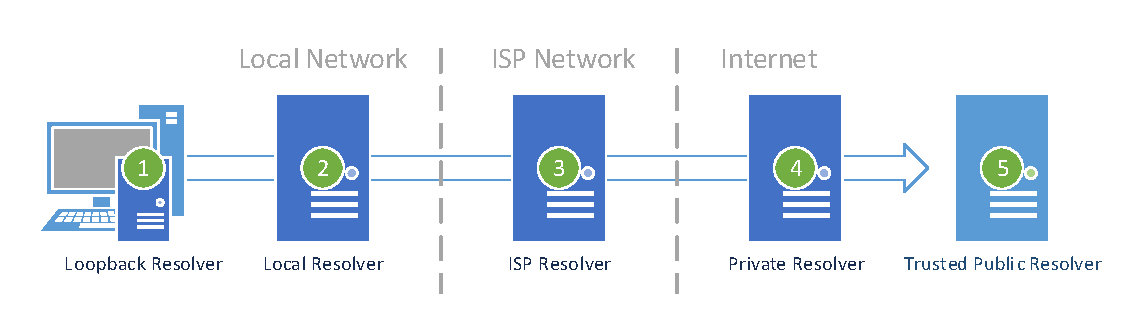
\includegraphics[width=\textwidth,trim={8mm 8mm 8mm 8mm},clip]{Impl_ResolverPositions}
    \caption{Stellt die möglichen Positionen eines Resolvers, aus Sicht des Clients, dar.}
    \label{img:impl-resolverpositions}
\end{figure}

\paragraph{Local-Loopback Resolver (1)}
Diese Position ist bei einem, auf die Verbindung zwischen Recursive Resolver und Stub-Resolver abgezielten, Angriff die sicherste. Werden Techniken wie DoT, DoH oder DNSCrypt im Forwarding Modus eingesetzt, kann darüber hinaus die Vertraulichkeit und Authentizität bis zum Recursive Resolver sichergestellt werden. Die Nachteile ist die fehlende Möglichkeit eines geteilten Caches, die erhöhte Ressourcenverbrauch am Client und der hohe Wartungsaufwand. Außerdem können keine Internet-Of-Things (IoT) Geräte bedient werden, da bei diesen eine Installation eines lokal laufenden Resolvers nicht möglich ist.

\paragraph{Local Network Resolver (2)}
Durch einen Resolver im Lokalen Netzwerk, besteht zwar die Gefahr von Angriffen auf Netzwerkebene, es wird jedoch der Einsatz eines gemeinsamen Caches möglich und eine hohe Geräte-Kompatibilität stakt verbessert. In kleinen, gut gesicherten Netzwerken kann dieses Angriffsszenario aufgrund des geringen Risikos in Kauf genommen werden. Angriffe von außen sind jedoch durchaus möglich und wahrscheinlich, sollte der Resolver nicht speziell geschützt werden.

\paragraph{ISP Resolver (3)}
Da, wie in Abschnitt \ref{sec:thread-priv} beschrieben, nicht auf die Verantwortlichkeit von ISPs oder staatlichen Institutionen vertraut werden sollte, ist das Nutzen eines ISP-Resolvers, vor allem in Hinblick auf Privacy, nicht zu empfehlen. Einzige Ausnahme stellt dabei der Einsatz von Technologien wir DNSCurve, EncDNS und ODNS dar, da diese eine Verschlüsselung der Anfragen durch den Resolver hindurch unterstützen. Aufgrund kurzer Laufwege und großen Caches sind diese Resolver in den meisten Fällen durchaus performant.

\paragraph{Private Resolver (4)}
Betreibt man seinen eigenen Resolver im Internet erhält man dadurch Kontrolle über die Privacy-Einstellungen des Resolvers. Abgesehen davon, setzt man sich damit jedoch allen möglichen Angriffen, nicht nur auf DNS, aus. Darüber hinaus sind die meisten Stub-Resolver nicht dazu in der Lage über sichere Protokolle mit dem Resolver zu kommunizieren. Abgesehen davon muss darauf geachtet werden, dass keine Zuordnung zwischen der Resolver-IP in einzelnen Personen hergestellt werden kann. Da diese Nachteile den Vorteilen stark überwiegen kann vom Einsatz eines eigener, privater Resolvers abgeraten werden.

\paragraph{Public Resolver (5)}
Der direkte Einsatz eines Trusted Public Resolvers hat viele Vorteile. Die Performance ist aufgrund guter Anbindungen, eines professionellen Betriebs und großen Caches meist gut. Viele Resolver haben spezielle Schutzmaßnahmen gegen Cache Poisoning- oder DoS-Attacken im Einsatz. Außerdem ist die Anonymität gegenüber autoritativen DNS-Servern, aufgrund der hohen Zahl an Users, als ausreichend anzusehen. Der einzige, schwerwiegende Nachteil besteht in der Gefahr von Privacy-Verletzungen durch den Betreiber des Dienstes. Hier ist entweder eine Abwägung zu treffen oder eine Lösung zur vollständigen Anonymisierung zu finden. 

\section{Technologie-Stack}
Zur Auswahl des Sets an Technologien (hier als ``Stack'' bezeichnet) wurde aufgrund der, am Ende des Kapitels \ref{chap:attacks} angeführten, Übersicht erstellt. Dabei wurde darauf geachtet, jede der unter \ref{chap:solutions} abgegebenen Empfehlungen gerecht zu werden. Um die Auswahl besser verstehen zu können, wird hier kurz auf jede einzelne der Techniken eingegangen.

\paragraph{DNSSEC}
DNSSEC stellt aktuell die einzige Möglichkeit zur Echtheitsprüfung von RRs selbst dar (siehe Abschnitt \ref{sec:tec-dnssec}). Das Abfragen und Validieren der \ac{DNSSEC} RRSig-Records ist somit Pflicht für jeden Resolver mit Sicherheitsfokus. Die Validierung kann an verschiedenen Stellen erfolgen. Da die Validierung aufgrund der kryptographischen Operationen durchaus ressourcenintensiv sein kann, ist es Sinnvoll diese Operation nicht auf jedem Client durchzuführen. Abgesehen davon fehlt vielen Stub-Resolvern die Möglichkeit zur selbstständigen Validierung. Wird ein Forwarding-Resolver eingesetzt, kommt es auf die Konfiguration und Implementierung an ob dieser eine Validierung durchführt oder sich auf den nachgeordneten Recursive Resolver verlässt. Kann dem rekursiven Resolver vertraut werden, ist die Verifizierung durch diesen, aus Effizienzgründen, zu bevorzugen.

\paragraph{DNS-over-TLS}
Wie in Abschnitt \ref{sec:tec-dot} beschrieben stellt DoT einen simplen Aufsatz zum klassischen DNS Netzwerkprotokoll dar. Für den Transport wird TLS über TCP auf Port 853 genutzt\cite{rfc7858}. Damit ist die Verbindung zwischen Resolver und Recursive Resolver geschützt. 

\paragraph{Address-Obfuscation über NAT}
Um auch die Vertraulichkeit der Anfragen erhalten zu können, kann zusätzlich der Zusammenhang zwischen der Client-Adresse und der Anfrage aufgelöst werden. Dies kann, wie schon in Abschnitt \ref{sec:tec-nat} erwähnt, durch den Einsatz eines NAT Servers erreicht werden. Zur Umsetzung kann nahezu jedes modernen Server-Betriebssystem herangezogen werden.

\section{Konzept}
Aus den beschriebenen Vor- und Nachteilen ergibt sich der Einsatz eines lokalen Forward-Resolver als optimaler Kompromiss aus Sicherheit, Kompatibilität und Performance. Der beschriebene Technologie-Stack ist in der Lage alle in Kapitel \ref{chap:solutions} vorgestellten Empfehlungen zu erfüllen. In Abbildung \ref{img:impl-architecture} wird der schematische Ablauf der Kommunikation gezeigt. Es werden dabei zusätzlich die Übergangsstellen der Verschlüsselung und Client-Identifizierbarkeit gezeigt.
\begin{figure}[hb]
    \centering
    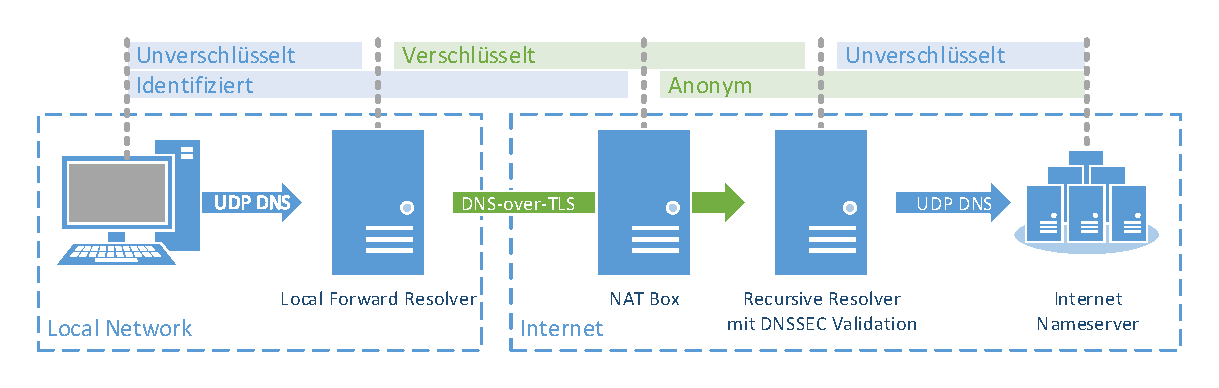
\includegraphics[width=\textwidth,trim={5mm 5mm 5mm 5mm},clip]{Impl_Architecture}
    \caption{Darstellung des schematischen Kommunikationsweg des Test-Aufbaus.}
    \label{img:impl-architecture}
\end{figure}

Um die Privacy der lokalen Clients und damit der Nutzenden zu wahren, wurde der Aufbau nach einem einfachen Grundkonzept entworfen: Entschlüsselte DNS-Nachrichten dürfen nur auf vom User direkt kontrollierten Komponenten mit der externen Internet-Adresse verknüpfbar sein. Dadurch wird verhindert, dass Betreiber der Transportnetzwerke oder der nachgeordneten DNS-Komponenten private Daten mit der Identität der Nutzenden verknüpfen.

Des weiteren wird durch DoT jede Form von Sniffing und Spoofing Attacken unmöglich gemacht. Da der Forwarding-Resolver selbst keine normalen DNS Anfragen von außerhalb des lokalen Netzwerks annimmt, ist der Resolver auch gegen DNS DoS Attacken durch externe Angreifer geschützt. Die \ac{DNSSEC} Validierung erfolgt je nach Implementation am lokalen Forward-Resolver oder am Public-Recursive-Resolver. Es ist damit selbst im Falle einer erfolgreichen Cache-Poisoning Attacke auf den Public Resolver nicht möglich RRs zu kompromittieren, die durch \ac{DNSSEC} Signaturen geschützt sind.

\section{Aufbau}
\label{sec:architecture}
Zu Validierung des Entwurfs wurde ein einfacher Testaufbau umgesetzt. Dieser verwendet Windows 10\footnote{Microsoft Windows Version 1803 (Build 17134.285)} als Test-Client-Betriebssystem und Fedora 28\footnote{Linux 4.17.19-200.fc28.x86\_64} als Betriebssystem des lokalen Resolvers. Der Local-Resolver selbst wurden zwecks Vergleichbarkeit mit zwei verschiedenen Software-Paketen umgesetzt: Unbound\footnote{Version 1.7.3 (kompiliert mit OpenSSL 1.1.0h-fips)} und Knot-Resolver\footnote{Version 2.4.1}. Als Trusted-Public-Resolver wurde das Quad9-Projekt gewählt da es DoT anbietet und einer zu befürwortende Privacy-Policy\cite{Quad9Privacy} folgt. Darüber hinaus werden Domänen, die in Zusammenhang mit Schadsoftware stehen, vom Quad9-Resolver automatisch geblockt. Dieses Feature kann zwar als Zensur verstanden werden, durch die aktuelle Bedrohung durch DNS unterstützte Malware \cite{Alcoy2017} und die strikt auf ``Phishing, Malware, and Exploit-Kits'' konzentrierte Sperrliste\cite{Quad9FAQ} kann die Bedrohung durch Zensur der durch Malware vorübergehend untergeordnet werden.   
\begin{wrapfigure}{r}{0.5\textwidth}
    \begin{center}
    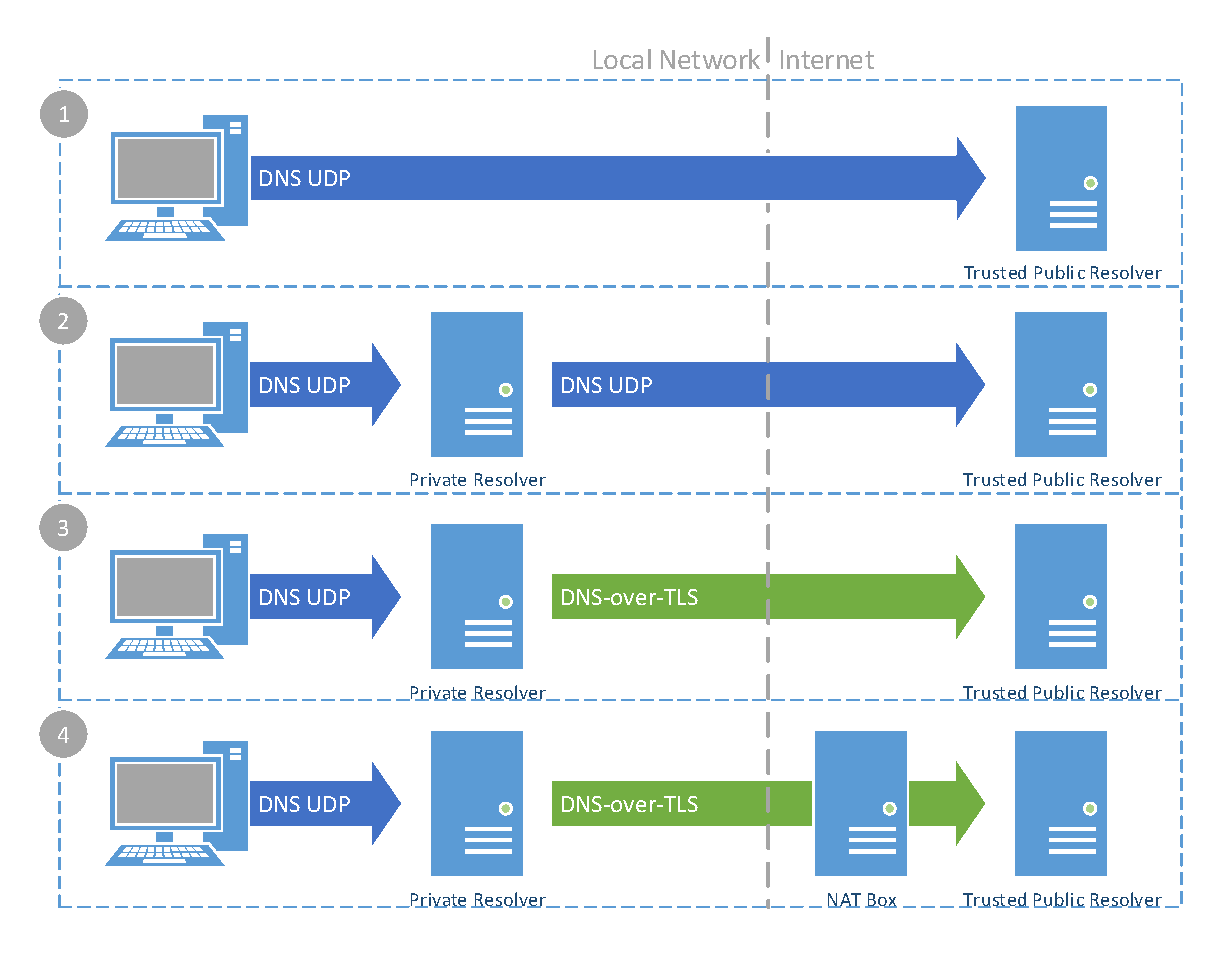
\includegraphics[width=0.48\textwidth,trim={5mm 8mm 5mm 8mm},clip]{Impl_Scenarios}
    \end{center}
    \caption{Darstellung der getesteten Szenarien}
    \label{img:impl-scenarios}
\end{wrapfigure}

Wie in Abbildung \ref{img:impl-scenarios} dargestellt wurden für den Performance- und Funktions-Test vier Szenarien gewählt. Dabei erfüllt nur Szenario 4 alle beschriebenen Schutzmechanismen, wobei Szenario 3 nur die Anonymität gegenüber des Public Resolver verletzt. Geht man von einem vertrauenswürdigen Anbieter dieses Resolvers aus, kann auf die Anonymisierung über den NAT-Server verzichtet werden. Wie man sieht, wird in jedem Fall von einem sicheren lokalen Netzwerk ausgegangen, mögliche Lösungen bei unsicheren Netzwerken wir in Kapitel \ref{chap:conclusion} diskutiert. 

\paragraph{Public-Resolver über UDP (1)}
Durch die direkte Verbindung zwischen Stub-Resolver und Public Resolver wird auf jegliche Vertraulichkeit der Übertragung verzichtet, da der in Windows integrierte Stub-Resolver keine Form der Verschlüsselung unterstützt. Abgesehen davon, ergibt sich durch die minimale Anzahl an Zwischenstellen eine optimale Latenzzeit, die sich positiv auf die gesamte Performance auswirkt.

\paragraph{Lokalen Forwarding-Resolver über UDP (2)}
In diesem Fall wird ein Forwarding-Resolver im lokalen Netzwerk installiert. Da dieser das klassische DNS-Netzwerkprotokoll zur Kommunikation mit dem Recursive-Resolver verwendet, ergibt sich noch kein Schutz der Vertraulichkeit. Mit einer restriktiven Konfiguration und verschiedenen, von der Implementation abhängigen, Sicherheitsfeatures können jedoch gewisse Arten von Spoofing-Attacken ausgeschlossen werden. Befindet sich eine Firewall an der Netzwerkkante so kann diese, durch den Einsatz eines lokalen Resolvers, sehr restriktiv Eingestellt werden. Dies verhindert direkte Angriffe auf Stub-Resolver von extern. Ein weiterer Vorteil besteht beim Einsatz von ``Knot-Resolver'' da dieser bestimmte DNS Rebinding Attacken (siehe \ref{sec:attack-dnsrebind}) abwehren kann, indem er interne IP-Adressen in Antworten verbietet\cite{KnotResolverDocRebinding}.

\paragraph{Lokaler Forwarding-Resolver mit DoT (3)}
Wird die Verbindung zum Recursive-Resolver nun durch ein Verschlüsselungsprotokoll wie DoT (siehe \ref{sec:tec-dot}) geschützt, ergibt sich ein klarer Vorteil: Es besteht eine sichere Verbindung zwischen dem Forwarding- und Recursive-Resolver, was Sniffing-, Spoofing-, sowie MITM-Attacken auf diesem Wege ausschließt. Durch den Einsatz von verbindungsorientierten Protokollen und Verschlüsselung werden jedoch der steigende Ressourcenverbrauch und höhere Latenzzeiten merkbar.

\paragraph{Lokaler Forwarding-Resolver mit DoT und NAT (4)}
Fügt man dem Aufbau nun einen NAT-Server (siehe \ref{sec:tec-nat}) hinzu, erhält man den Vorteil der Anonymität gegenüber des Recursive-Resolvers. Da dies der einzige Vorteil des Aufbaus darstellt, ist die dadurch einhergehende Erhöhung der Latenzzeit gegen den Schutzbedarf abzuwägen.

\section{Tests und Messungen}
\label{sec:measurements}
Die Kontrolle der unter \ref{sec:architecture} beschriebenen Varianten wurde nun mithilfe der Programme dig\footnote{Auf Ubuntu Subsystem for Windows10; DiG 9.10.3-P4-Ubuntu} sowie ``DNS Benchmark''\footnote{von Steve Gibson Version 1.3.6668.0} durchgeführt. Gemessen wird die gesamte benötigte Umlaufzeit (Round-Trip-Time; RTT) 100 ungecachter, zufälliger Einträgen. Die gewählten Konfigurationen der DNS-Server sind in \nameref{chap:appA} zu finden und wurden nach den offiziellen Dokumentationen und darin enthaltenen Sicherheitsempfehlungen erstellt. Als ``Hardware'' wurden 3 virtuelle Maschinen (1 vCPU, 1GB RAM) auf einem vom Test-Client unabhängigen Host genutzt. Um eine optimale Vergleichbarkeit der einzelnen Varianten zu erreichen wurden die Tests der Performance von einem Test-Client auf die 3 Server simultan durchgeführt. Dabei wurden in 2 unabhängigen Läufen alle unterschiedlichen Varianten einer Software getestet. In einem dritten Lauf wurde die direkte Performance von 25 offener DNS-Resolvern (siehe \ref{chap:appB}) getestet und die 10 besten zur Errechnung der direkten Vergleichswerte herangezogen. Für die Auswertungen wurden immer nur Werte von ungecachten Einträgen herangezogen, da nur diese eine Kommunikation mit dem Recursive-Resolver verlangen. Die Ergebnisse der Tests sind unter Kapitel \ref{chap:results} angeführt. 



\chapter{Ergebnisse}
\label{chap:results}

Die in Abschnitt \ref{sec:measurements} beschriebenen Messungen der Umlaufzeiten (Round-Trip-Times;RTT) verschiedener DNS-Anfragen ergaben die in Abbildung \ref{img:results-times} dargestellten Zeiten. Aus diesen Werten ergeben sich nun folgende Ergebnisse.

\paragraph{Performance Einbußen durch DoT}
Wie schon in Kapitel \ref{chap:implementation} näher ausgeführt, war ein Performanceverlust durch den Einsatz von DoT zu erwarten. Dieser schlägt sich speziell in den Minimalzeiten mit ca. 50-100\% Erhöhung nieder. Dies ist auf den notwendigen Verbindungsaufbau zurückzuführen. Diese Werte decken sich grob mit den früheren Messwerten aus der Arbeit von Zhu et al.\cite{Zhu2015} und zeichnen sogar ein etwas besseres Bild. Die durchschnittlichen RTTs der herkömmlichen DNS-Abfragen über UDP betragen dabei 105ms, wobei die über TLS mit 115-128ms um ca. 20\% erhöht sind.

\paragraph{Auswirkung des NAT-Servers}
Vergleicht man nun die Werde der Variante mit und ohne Anonymisierung mittels NAT so erkennt man nur minimale Unterschiede. Ja nach Implementation wurde Unterschiede von 5-11ms beobachtet, was bei einer Gesamtdauer von ca. 120ms 5-9\% ausmacht. Da es zu den alternativen Anonymisierungstechnologien EncDNS und ODNS keine aktuellen Implementierungen gibt, kann dieser Zeitverlust mit keiner Alternative verglichen werden.

\begin{figure}[hb]
    \centering
    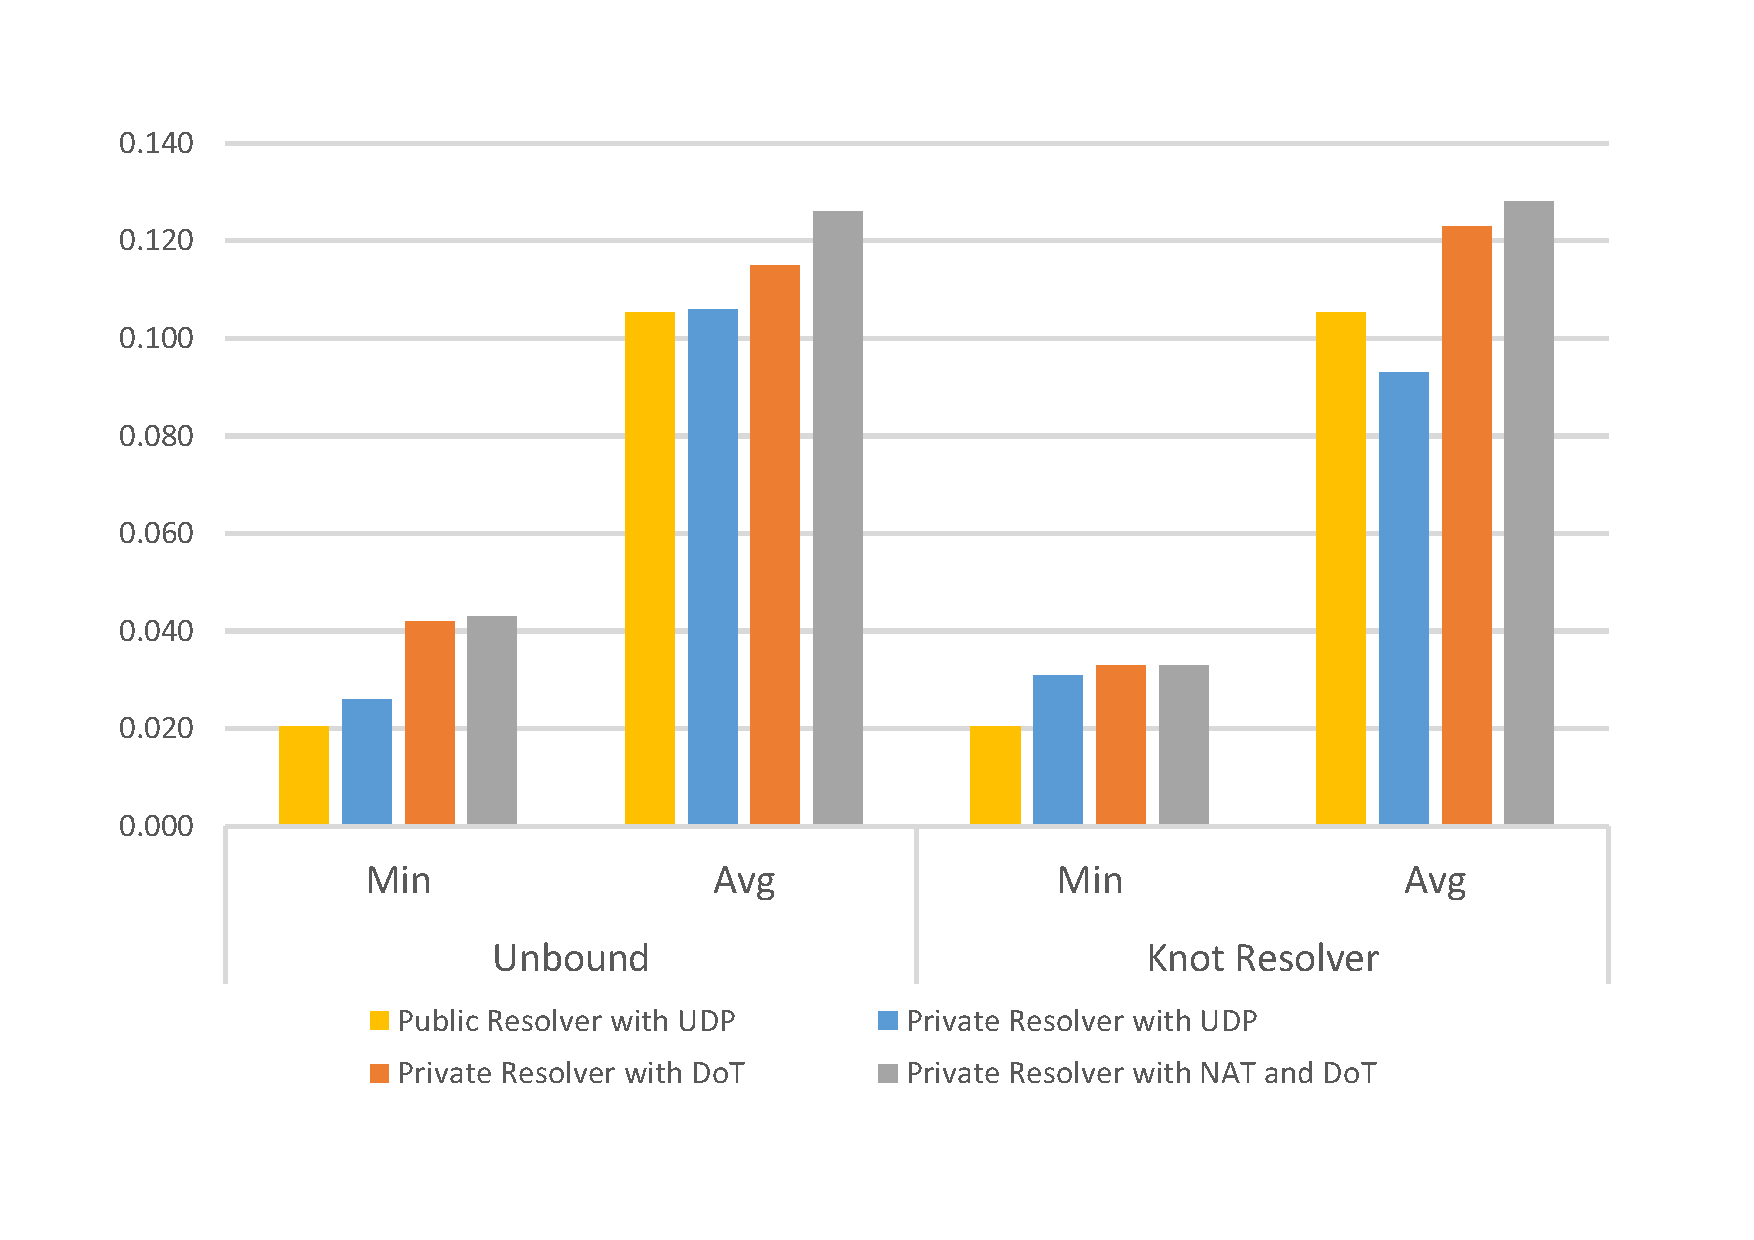
\includegraphics[width=0.6\textwidth]{Results_ResponseTimes}
    \caption{Balkendiagramm der Umlaufzeiten von DNS-Anfragen bei verschiedenen varianten des dargelegten Aufbaus. Die Werte sind in Sekunden angegeben. Die Minimal- (min.) und Durchschnittswerte (avg.) ergeben sich aus Messungen mit dem Programm ``DNS Benchmark'' von Steve Gibson}
    \label{img:results-times}
\end{figure}

\chapter{Ergebnis}
\lipsum

%\section{Allgemeine Empfehlungen}

%\subsection{DNSSEC}

%\subsection{DNS-over-TLS}
%\subsection{Server- / Netzwerkaufbau}
%\subsection{Netwerksetup}
%\subsection{Vertrauenswürdige Resolver / Upstream-DNS Server od. IDS}

% *Nur mit entsprechender Validierung des Zeilservers (DoT, etc.) weil sonst anfällig auf MitM, BGP-Hijacking, usw.*

%\section{Konkrete Konzepte}

%\subsection{Enterprise: local-only DNS-Resolver mit DNSSEC und IDS, HTTP-Proxy for Clients/internal Servers}

%\subsection{Privat/EPU: DNS-over-TLS  mit Trusted Resolver (z.B. Stubby and Quad9)}

% Keine gute Privicy trotz Encryption weil kein padding und timing attacken (Siby und Shulman). 

\chapter{Ausblick}
\label{chap:future}

% Wenn DNSSEC große Durchdringung hat => MitM Problem weg
% Wenn T-DNS anklang findet DoS, Spoofing und Poisoning von Servers wenig problematisch
% Wenn DoT in OS und DoH in alle Browser integriert wird kein Problem mehr auf "letzter Meile" 
% Sonst DNSCrypt/DoT als Schutz zwischen Stub-Resolver und Forwarding-Resolver

\lipsum

% Literaturverzeichnis
\bibliography{literatur} 
\bibliographystyle{ieeetr}
\clearpage

% Abbildungsverzeichnis
\listoffigures
\clearpage

% Tabellenverzeichnis
\listoftables
\clearpage

% Verzeichnis der Listings
\lstlistoflistings
\clearpage

% Abkürzungsverzeichnis
\phantomsection
\addcontentsline{toc}{chapter}{Abkürzungsverzeichnis}
\chapter*{Abkürzungsverzeichnis}
\begin{acronym}[XXXXX]
    \acro{ABC}[ABC]{Alphabet}
    \acro{WWW}[WWW]{world wide web}
    \acro{ROFL}[ROFL]{Rolling on floor laughing}
\end{acronym}

%Anhänge
\chapter*{Anhang A}
\label{chap:appA}
In diesem Anhang werden die für die Reproduktion notwendigen Konfigurationsdateien zur Verfügung gestellt. 

Das Nachfolgende Listing stellt das Konfigurationsscript für die Host-Firewall des Servers dar. Es wurde dabei ein minimales Setup gewählt. Dabei sind nur die notwendigen ein- und ausgehenden Verbindungen berechtigt.

\lstinputlisting[language=Bash]{code/set-fw.sh}
\clearpage

Die Konfigurationsdatei \texttt{/etc/unbound/unbound.conf} des Unbound 1.4.7 Servers ist in folgendem Listing festgehalten. Die Kommentare ab Zeile 41 stellen dabei die einzelnen Betriebsmodi dar. Zum aktivieren einfach die aktuellen Zeilen aus- und die anderen einkommentieren.   

\lstinputlisting[language=Bash]{code/unbound.conf}
\clearpage

Diese Listing foltg dem von oben, betrifft hier nur die Knot-Resolver-Config unter \texttt{/etc/knot-resolver/}.

\lstinputlisting[language={[5.0]Lua}]{code/kresd.conf}

%spellcheck-off
\chapter{Anhang B}
\label{chap:appB}

Die nachfolgende Tabelle zeigt die Rohdaten der Messergebnisse der Software ``DNS Benchmark''. Die Zahlenwerte zeigen die minimale (min), durchschnittliche (avg) und maximale (max) RTT, sowie deren Standardabweichung (Std.Dev) sowie die Erfolgsrate von 10 ausgewählten Open-Recursive-Resolvern. Diese Werte wurden als Durchschnitte zur Errechnung eines Vergleichswerts für die in Kapitel \ref{chap:results} vorgestellten Ergebnisse verwendet.

\begin{table}[ht]
\centering
\caption{Daten aus der Vergleichswertemessung}
\begin{tabular}{lllllll}
\hline
Resolver IP    & Min   & Avg   & Max   & Std.Dev & Reliab\% \\ \hline
129.250.35.250 & 0.009 & 0.012 & 0.022 & 0.002   & 100.0    \\
129.250.35.251 & 0.009 & 0.012 & 0.017 & 0.001   & 100.0    \\
1.1.1.1        & 0.009 & 0.013 & 0.017 & 0.002   & 100.0    \\
9.9.9.9        & 0.010 & 0.013 & 0.023 & 0.002   & 100.0    \\
1.0.0.1        & 0.014 & 0.017 & 0.023 & 0.002   & 100.0    \\
8.8.8.8        & 0.016 & 0.019 & 0.024 & 0.002   & 100.0    \\
8.8.4.4        & 0.015 & 0.019 & 0.027 & 0.002   & 100.0    \\
4.2.2.4        & 0.021 & 0.024 & 0.029 & 0.002   & 100.0    \\
4.2.2.6        & 0.021 & 0.024 & 0.030 & 0.002   & 100.0    \\
4.2.2.1        & 0.021 & 0.026 & 0.032 & 0.003   & 100.0    \\ \hline
\end{tabular}
\end{table}

\end{document}